%\documentclass[12p]{article}
%\usepackage{a4paper,makeidx}
%\usepackage[dvips]{graphics}
\documentclass{article}
\usepackage{graphicx}
\usepackage{subfig}
\usepackage{multirow}
\usepackage{float}
%\documentclass[smallextended]{svjour3}
%\usepackage[dvips]{graphicx}
%\usepackage{subfig}
%%%%%%%%%%%%%%%%%%%%%%%%%%%%%%%%%%%%%%%%%%%%%%%%%%%%%%%%%%%%%%%%%%%%%%%%%%%%%%%%%%%%%%%%%%%%%%%%%%%%%%%%%%%%%%%%%%%%%%%%%%%%

\righthyphenmin=55
\newlength{\gnat}
\newlength{\figheight}
\newlength{\figwidth}
\setlength{\textwidth}{6in}
\setlength{\evensidemargin}{0.2in}
\setlength{\oddsidemargin}{0.2in}
\setlength{\topmargin}{0.0in}
\setlength{\textheight}{9in}
\setlength{\headsep}{10pt}
\setlength{\columnsep}{0.375in}

\newtheorem{theorem}{Theorem}
\newtheorem{proposition}{Proposition}
\newtheorem{lemma}{Lemma}
\newtheorem{corollary}{Corollary}
\newtheorem{definition}{Definition}
\newtheorem{remark}{Remark}
\newtheorem{claim}{Claim}

\def\IR{\Bbb R}
\def\tF{{\tilde F}}
\def\tG{{\tilde G}}
\def\tE{{\tilde E}}
\def\hF{{\hat F}}
\def\hG{{\hat G}}
\def\hE{{\hat E}}
\def\oF{{\overline{F}}}
\def\oG{{\overline{G}}}
\def\CC{{\cal C}}
\def\uF{{\underline{F}}}
\def\uG{{\underline{G}}}
\def\oC{{\overline{C}}}
\def\uC{{\underline{C}}}
\baselineskip= 20pt
%\input{tcilatex}
\graphicspath{ {Paper_figs/} }



\begin{document}

\date{}

%\big

\title {Random time transformation analysis of Covid19 2020
}

\author {
Isaac Meilijson
\\
{Tel-Aviv University} \\
\\
{Seminario en la Universidad de Chile, 18 de Junio de 2020}
}


%\titlerunning{Covid19 2020}
%\authorrunning{Alon and Meilijson}

\maketitle

\pagenumbering{arabic}

\bigskip

\begin{center}

\noindent Joint work with {\bf Nitay Alon}

\end{center}

\newpage

%\huge

%\section{Introduction} \label{introduction}

\noindent {\bf The SIR epidemiological model - Kermack \& McKendrick 1927}.

\bigskip

\noindent Susceptible cases $S(t) = K - X(t)$

\noindent Affected cases $X(t)$

\noindent Asymptote $K$, maximal $X$ (perhaps population size $N$)

\noindent Removed cases $R(t)$, dead or recovered

\noindent Infected cases $I(t)=S(t)-R(t)$

\begin{eqnarray}
dX(t) & = & \beta(t) g(I(t)) (1 - X(t)/K) dt \nonumber \\
dR(t) & = & \gamma I(t) dt \nonumber \\
I(t) & = & X(t)-R(t) \nonumber
\end{eqnarray}

\noindent where $K=N$ and $g(x)=x$.

\bigskip

\noindent {\bf Basic reproduction number} $R_0={\beta(t) \over \gamma}$ passage below $1$ indicates transition from increasing to decreasing $I(\cdot)$

\newpage

\noindent Covid19 2020 SIR may accept almost exact solution with $\beta$ (besides $\gamma$) constant, provided $g(x)=x^\alpha$
for some $\alpha<1$ (Bj{\o}rnstad, Finkenst\"{a}dt and Grenfell 2002) and $K$ free parameter.

\bigskip

\noindent {\bf Exponential or asymptotically linear growth?} $\alpha=1$ and $\alpha<1$ differentiate between exponential and sub-exponential growth for infinite population.

\bigskip

\noindent $\alpha=1$ equations: exponential growth. $d I(t) = (\beta-\gamma) I(t) dt$ derived from
\begin{eqnarray}
d X(t) & = & \beta (X(t)-R(t)) dt \nonumber \\
d R(t) & = & \gamma (X(t)-R(t)) dt \nonumber
\end{eqnarray}

$$
I(t)=I(0)\exp\{(\beta-\gamma)t\} \ ; \ (t)=X(0)\exp\{\beta t\} \ , \ R(t)=R(0)\exp\{\gamma t\}
$$

\bigskip

\noindent $\alpha<1$ equations: linear growth. $d I(t) = (\beta I(t)^\alpha - \gamma I(t))dt$ derived from
\begin{eqnarray}
dX(t) & = & \beta (X(t)-R(t)^\alpha dt \nonumber \\
dR(t) & = & \gamma (X(t)-R(t)) dt \nonumber
\end{eqnarray}

\noindent admits constant solution $I(t) \equiv I_0 = ({\beta \over \gamma})^{1 \over {1-\alpha}}$ with
$$
X(t) \approx X(0)+{{\beta^{1 \over {1-\alpha}}} \over {\gamma^{\alpha \over {1-\alpha}}}} t  \ ; \ R(t) \approx R(0)+{{\beta^{1 \over {1-\alpha}}} \over {\gamma^{\alpha \over {1-\alpha}}}} t
$$


\newpage

\noindent But population size is finite, and target sub-population may be small.

\bigskip

\noindent If $g(x)=x^\alpha$ with $\alpha<1$ and $K$ fitted with $\alpha, \beta, \gamma$, solutions invariably show typical Covid19 behavior of empirical data, number of infected cases $I(t)$ that increase to a maximum and then decrease, towards zero hopefully.

\bigskip

\noindent Profile likelihood function of alpha (Murphy and Van Der Vaart 2000) generally quite flat, $\alpha$ somewhat noisily estimated. But definitely in $(0,1)$.

\bigskip

\noindent End of May 2020 most countries and the world as a whole displayed $I(\cdot)$ increasing with time, making estimation more speculative than for countries where the basic reproduction number $R_0$ crossed already below $1$.

\bigskip

\noindent Quite popular to welcome $R_0$ transition, wrongly referred to as leaving behind exponential growth in favor of a period of recovery.

\bigskip

\noindent Transition occurs when number of infected cases is maximal, where care should be perhaps strengthened rather than relaxed.

%All graphs in the sequel show that the recovery period until the number of infected cases is at a safer low level "in the current wave", is long and slow.  The USA is at the transition point in early June, but if conditions stay stationary, the current wave is predicted to be still at unsafe levels in November. Germany and Italy are predicted to experience unsafe levels at least until the end of August.

\newpage

\begin{figure}
	\begin{center}
	%\subfloat [Second-chance model and absolute standard normal]
	{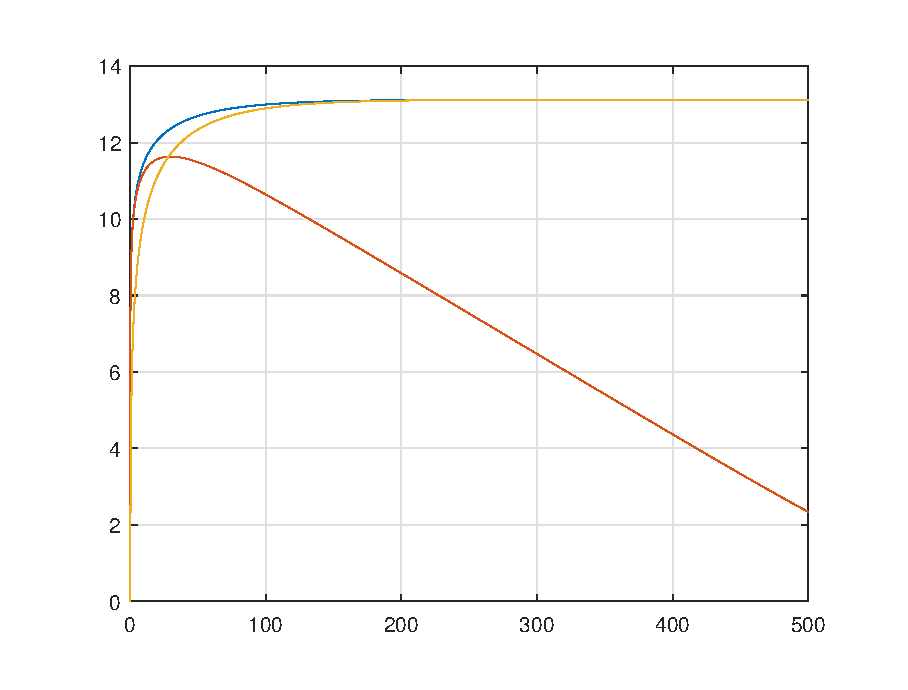
\includegraphics[width=1.5in,height=1.5in]{logalphazero.eps}}
	\qquad
	{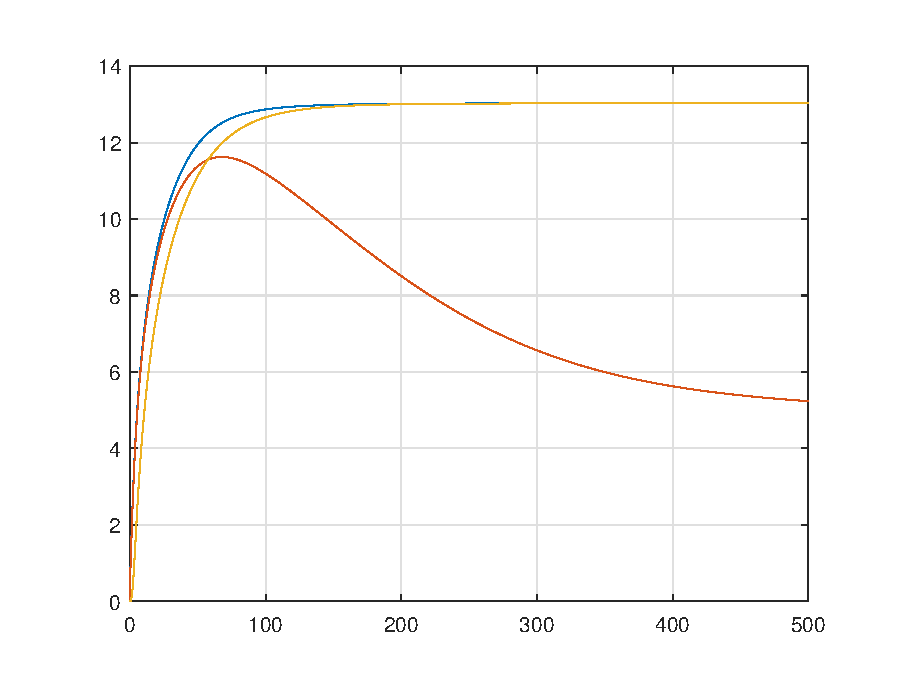
\includegraphics[width=1.5in,height=1.5in]{log075.eps}}
	\qquad
	{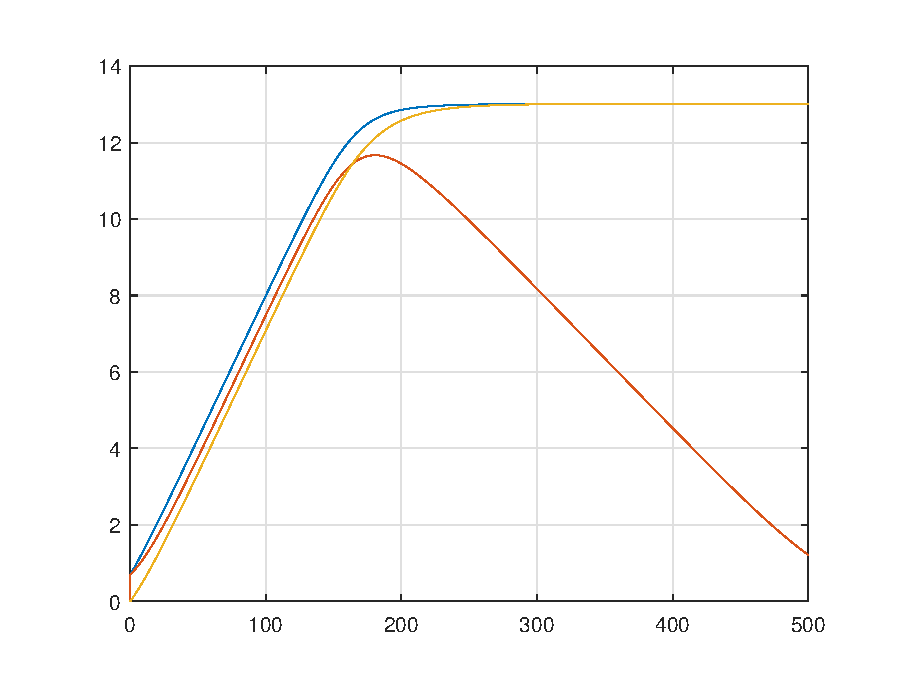
\includegraphics[width=1.5in,height=1.5in]{log1.eps}}
	%{\includegraphics[width=2in,height=2in]{Fig3.eps}}
	\end{center}
	%\begin{center}
	\caption{Log $X, I, R$ for $\gamma=0.05 , K=.5M$. $\alpha=0 , \beta=10000$. $\alpha=0.75 , \beta=2$. $\alpha=1 , \beta=0.125$}
	%\end{center}
	%\label{log075}
\end{figure}

\bigskip

\begin{figure}
\begin{center}
%\subfloat [Second-chance model and absolute standard normal]
{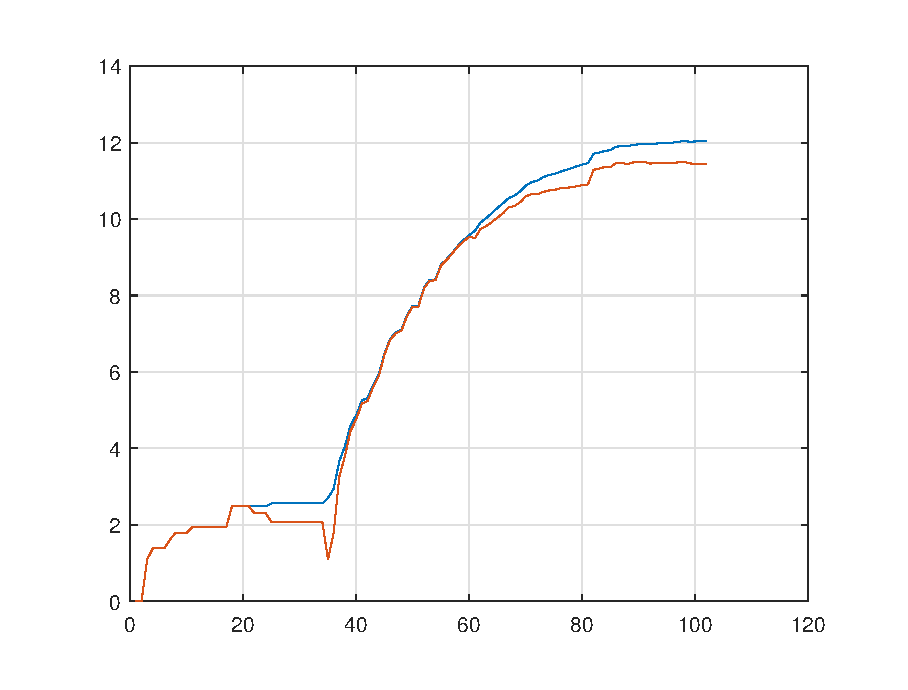
\includegraphics[width=1.5in,height=1.5in]{francelog.eps}}
 \qquad
{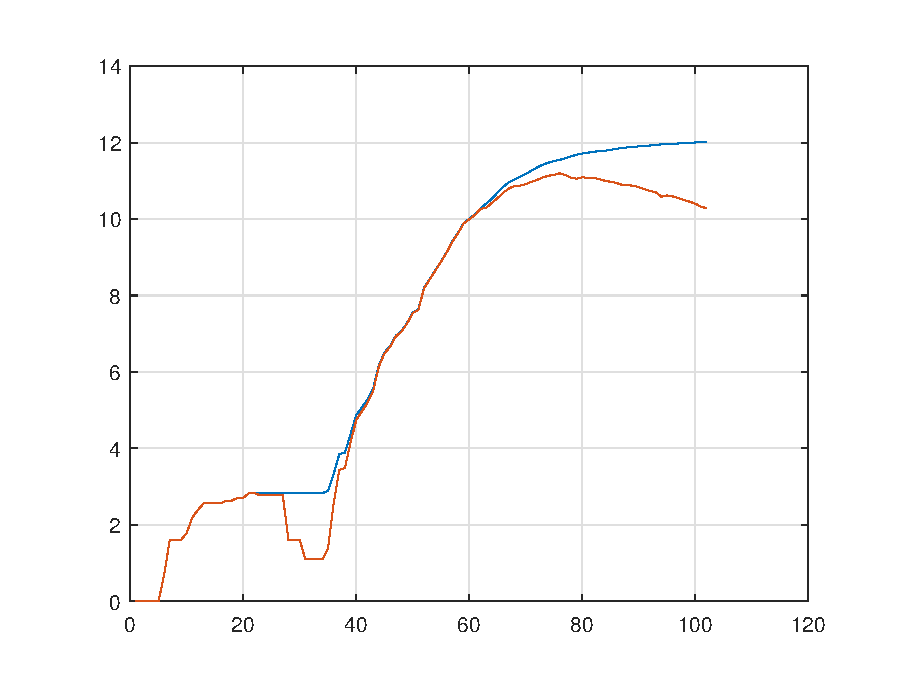
\includegraphics[width=1.5in,height=1.5in]{germany.eps}}
 \qquad
{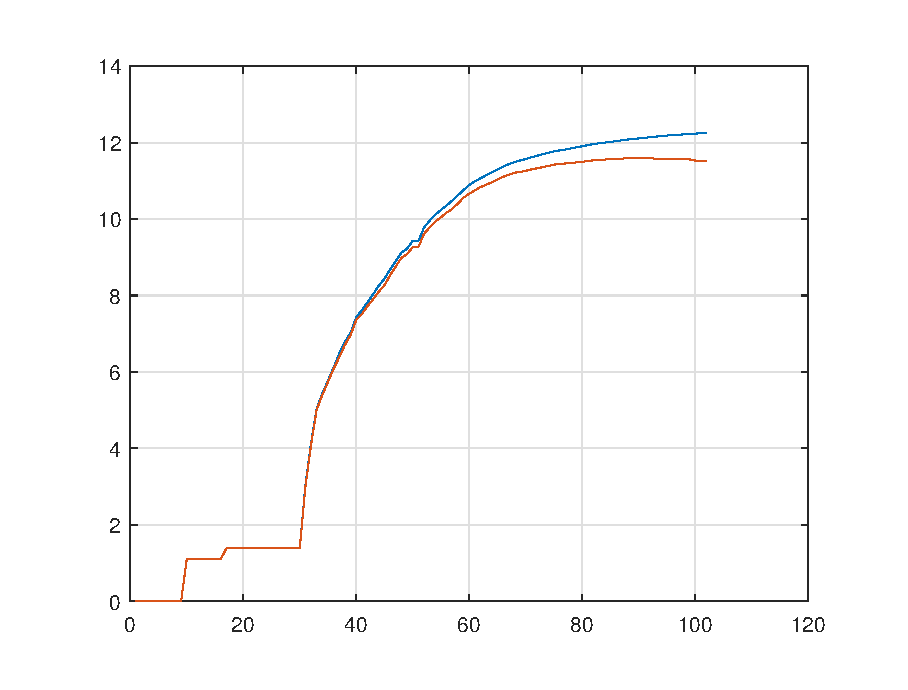
\includegraphics[width=1.5in,height=1.5in]{italy.eps}}
%{\includegraphics[width=2in,height=2in]{Fig3.eps}}
\end{center}
%\begin{center}
\caption{Logarithm of $X, I$, March to June 2020. L: France. M: Germany. R: Italy}
%\end{center}
%\label{france}
\end{figure}


\newpage
	
\noindent {\bf Preliminary data handling - empirical data $X, I, R$ and $\beta$}

\bigskip

\noindent New removed cases proportional to number of infected cases.

\bigskip

\noindent $R$ should be proportional to cumulative sum of $I$.

\bigskip

\noindent Linear regression with slope $\gamma$ and zero intercept should manifest this relationship.

\bigskip

\noindent Empirically measured $X$ kept intact but its split into $R$ and $I$ modified minimally so that the regression relation will hold.

\bigskip

\noindent $B$ is $n$ by $n$ matrix with $0$ above diagonal and $1$ on and below diagonal.

\noindent $A$ is $2 n$ by $n$ matrix with $\gamma B$ in first $n$ rows and $\gamma B$ plus identity matrix in last $n$ rows.

\noindent $V$ is column vector with $R$ in top half and $X$ in bottom half.

\bigskip

\noindent Regression equation $A \hat{I} \approx V$ gives "regression coefficients" $\hat{I}$ that are a compromise to manifest the requirement.

\newpage

\begin{figure}
\begin{center}
%\subfloat [Second-chance model and absolute standard normal]
{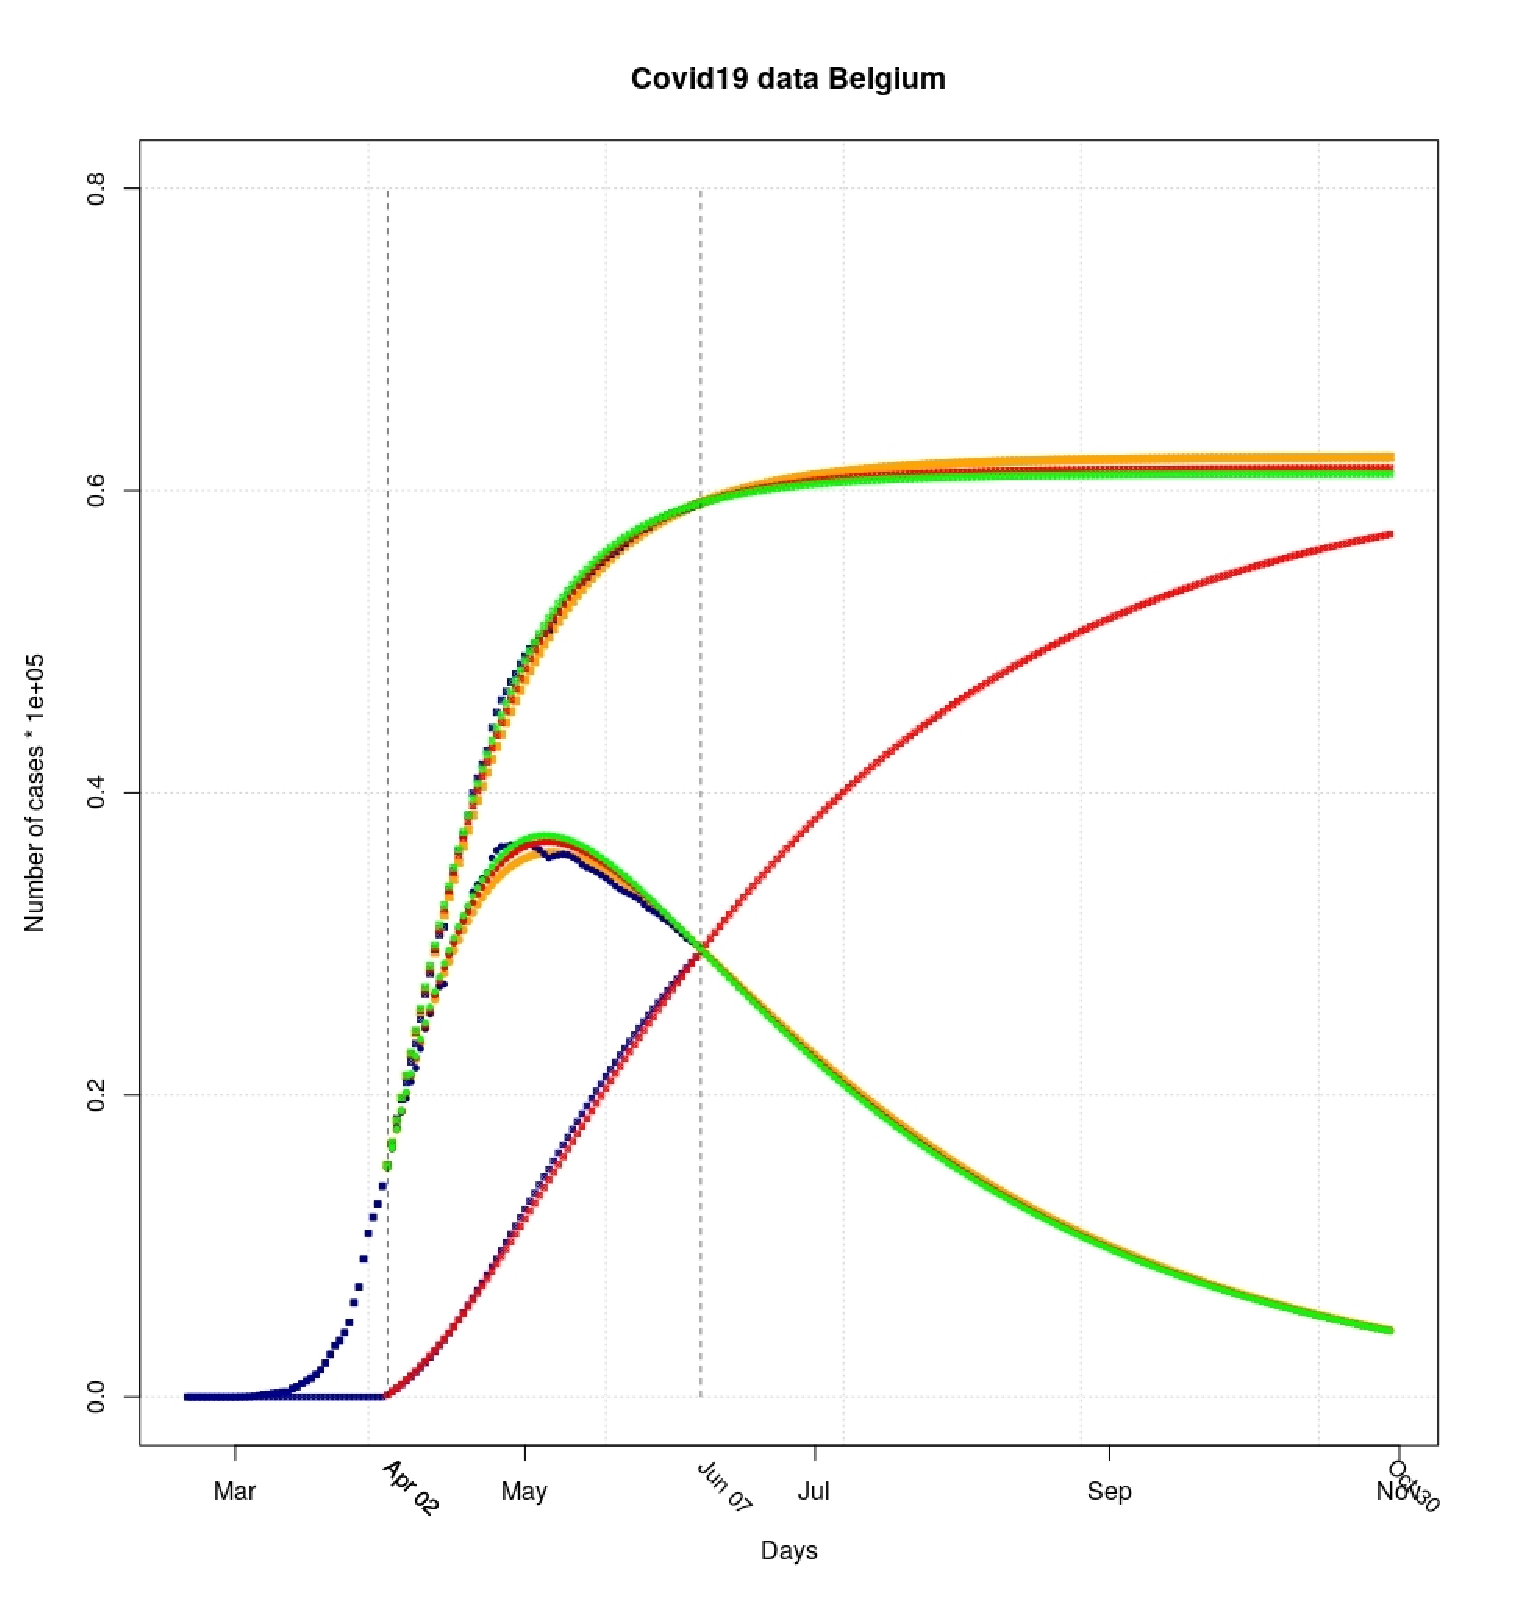
\includegraphics[width=2.5in,height=2in]{belgium_figure_a_07_06_2020.eps}}
\qquad
{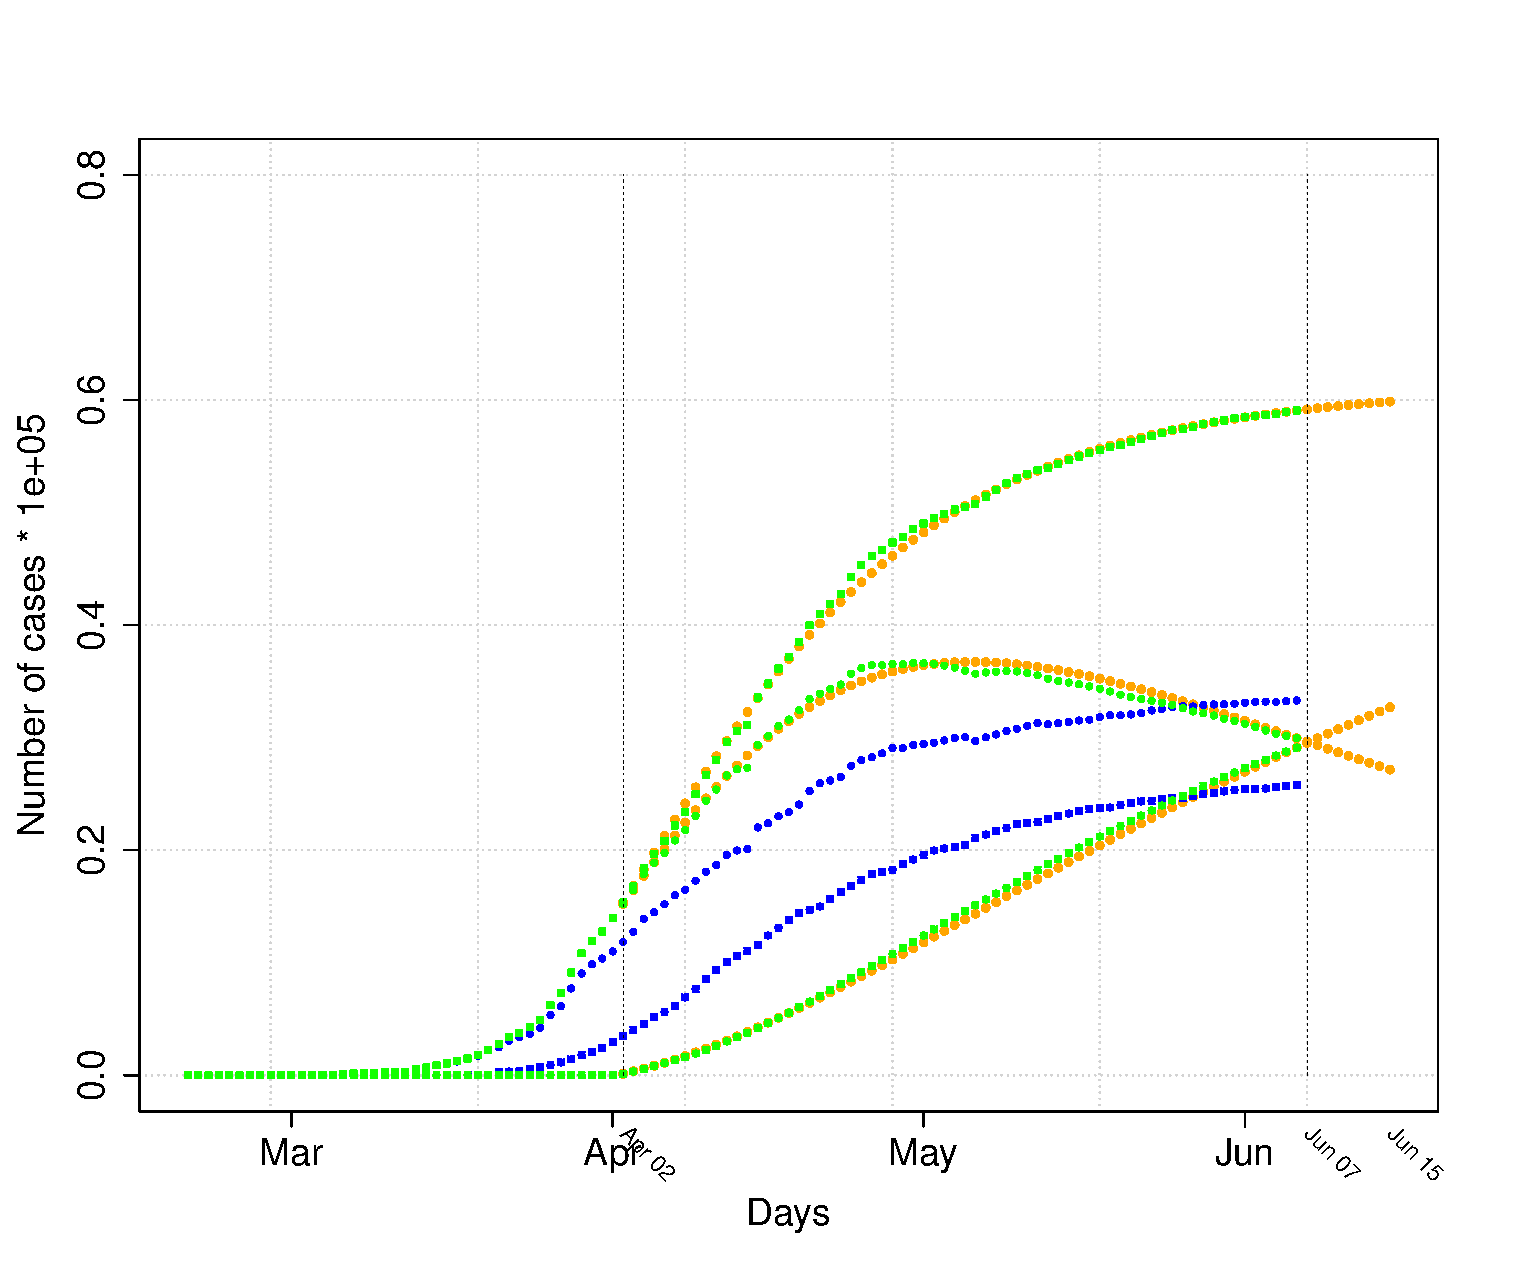
\includegraphics[width=2.5in,height=2in]{belgium_figure_b_07_06_2020.eps}}
\end{center}
\begin{center}
\caption{SIR model, data pre-processing and RTT solution, Belgium, March to June 2020
}
\label{fig:belgium_sir_model_07_06_2020}
\end{center}
\end{figure}


\begin{figure}
\begin{center}
%\subfloat [Second-chance model and absolute standard normal]
{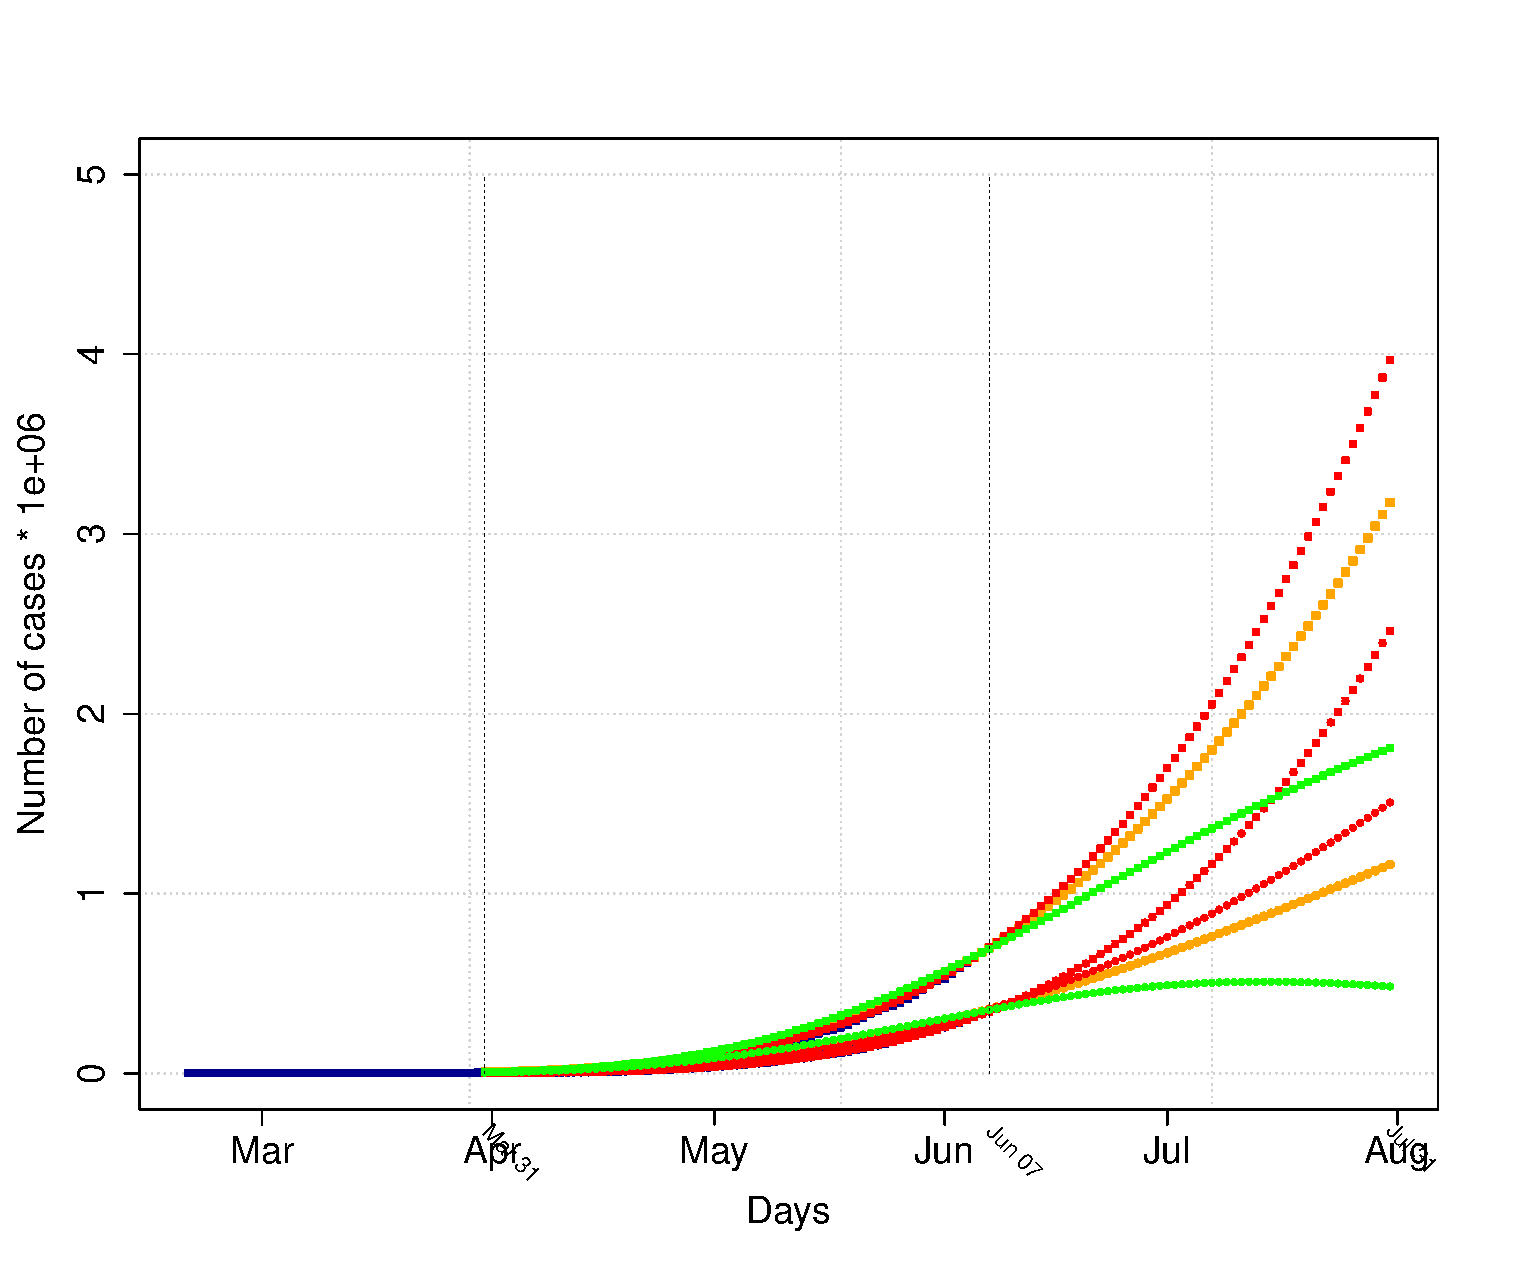
\includegraphics[width=2.5in,height=2in]{brazil_figure_a_07_06_2020.eps}}
\qquad
{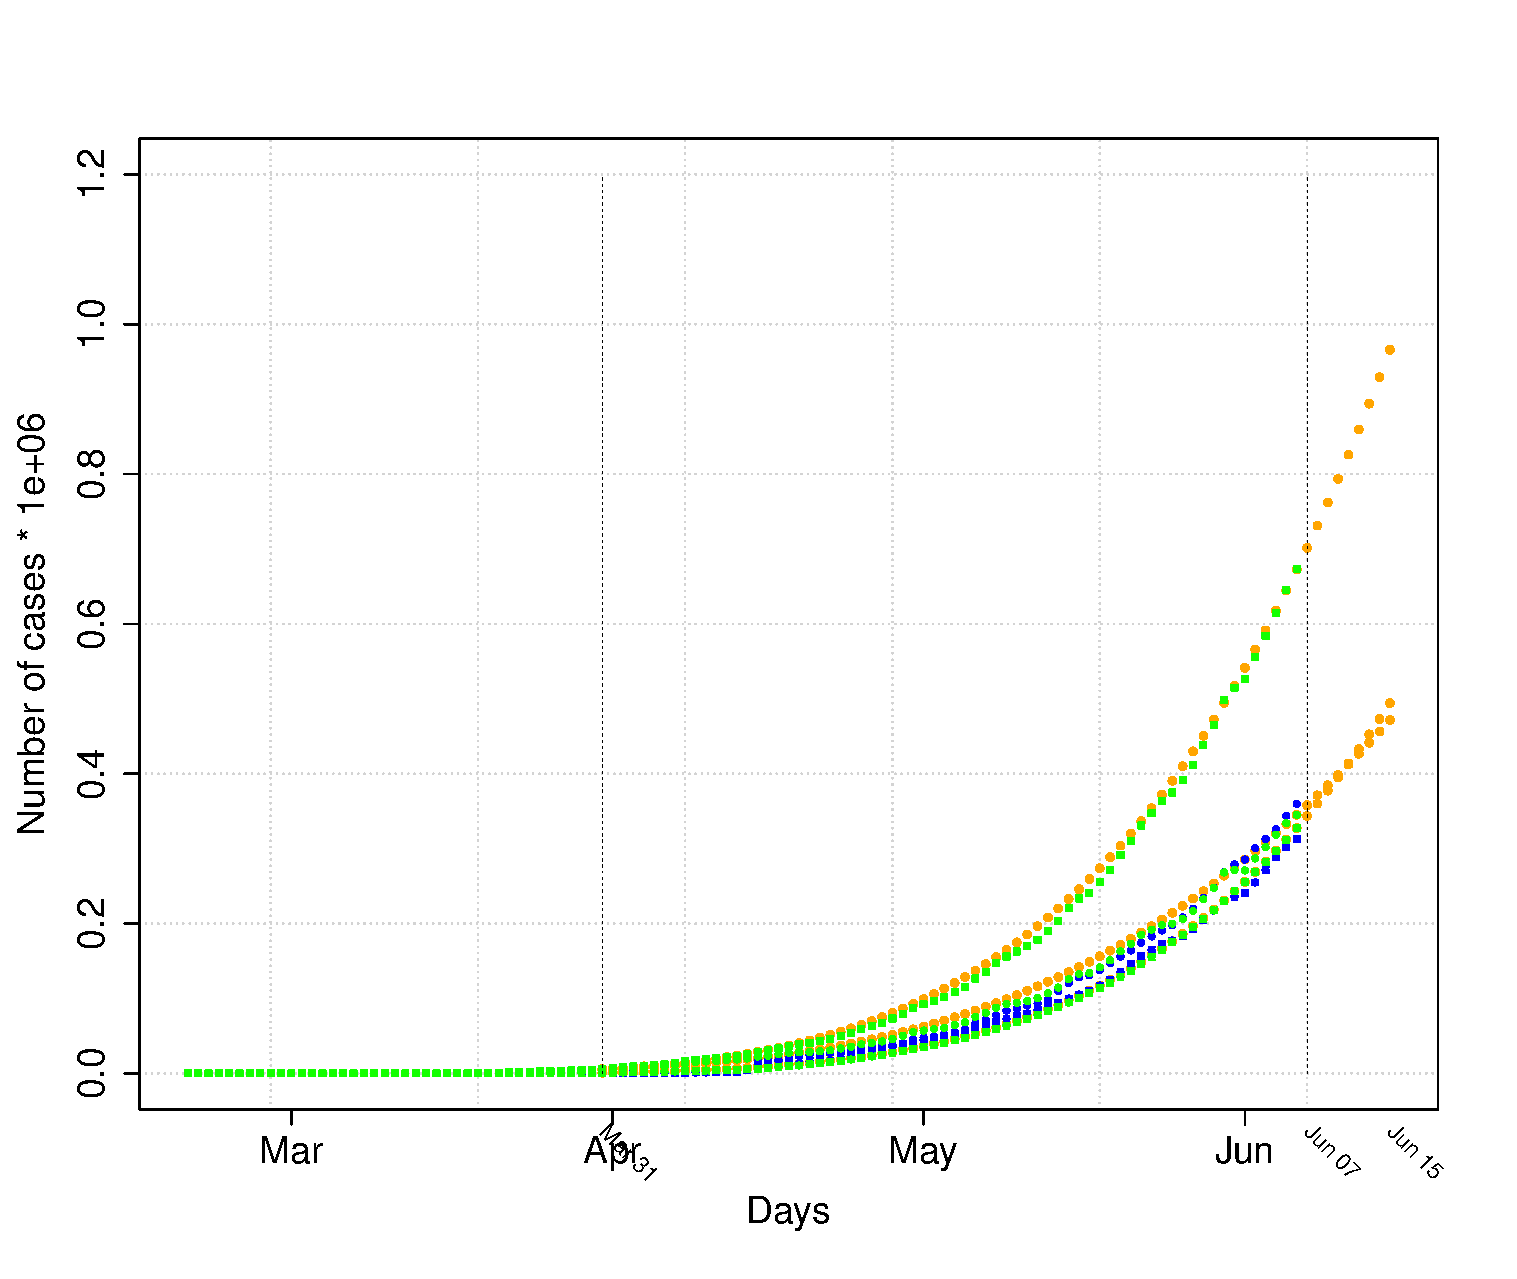
\includegraphics[width=2.5in,height=2in]{brazil_figure_b_07_06_2020.eps}}
\end{center}
\begin{center}
\caption{SIR model, data pre-processing and RTT solution, Brazil, March to June 2020
}
\label{fig:brazil_sir_model_07_06_2020}
\end{center}
\end{figure}


\begin{figure}
\begin{center}
%\subfloat [Second-chance model and absolute standard normal]
{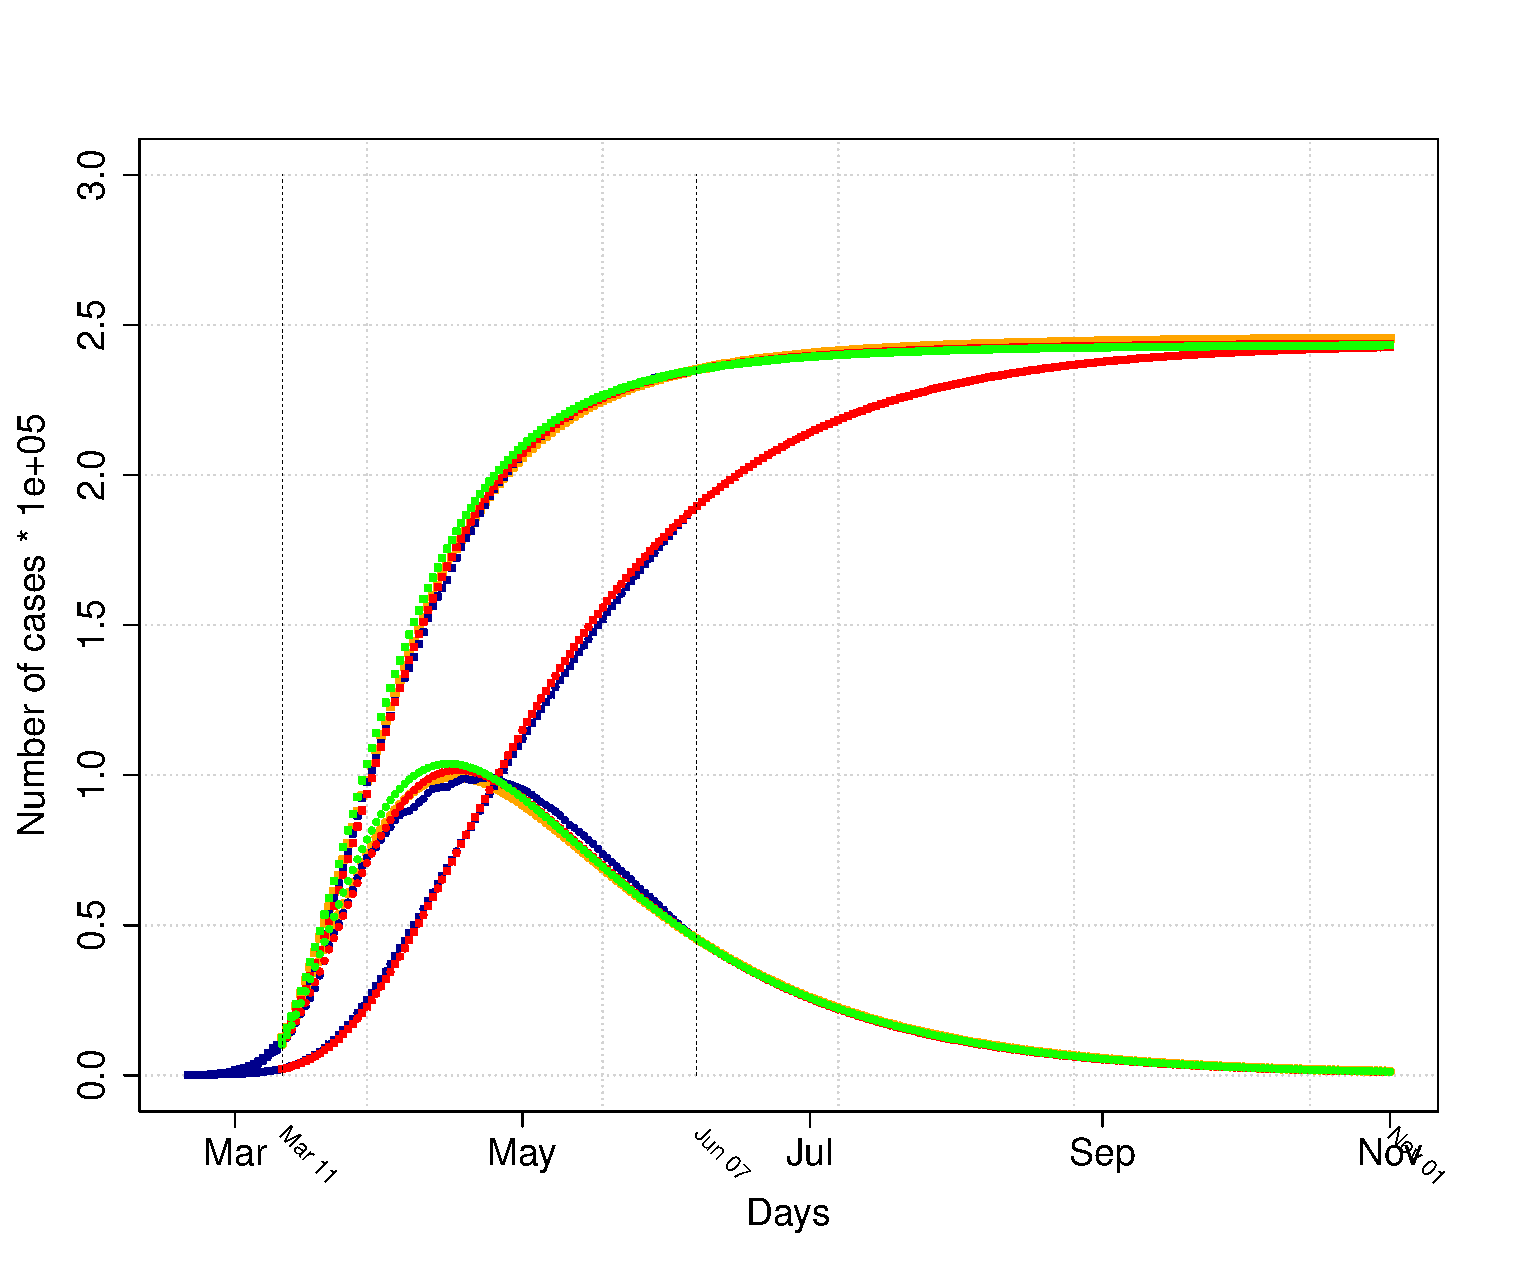
\includegraphics[width=2.5in,height=2in]{italy_figure_a_07_06_2020.eps}}
\qquad
{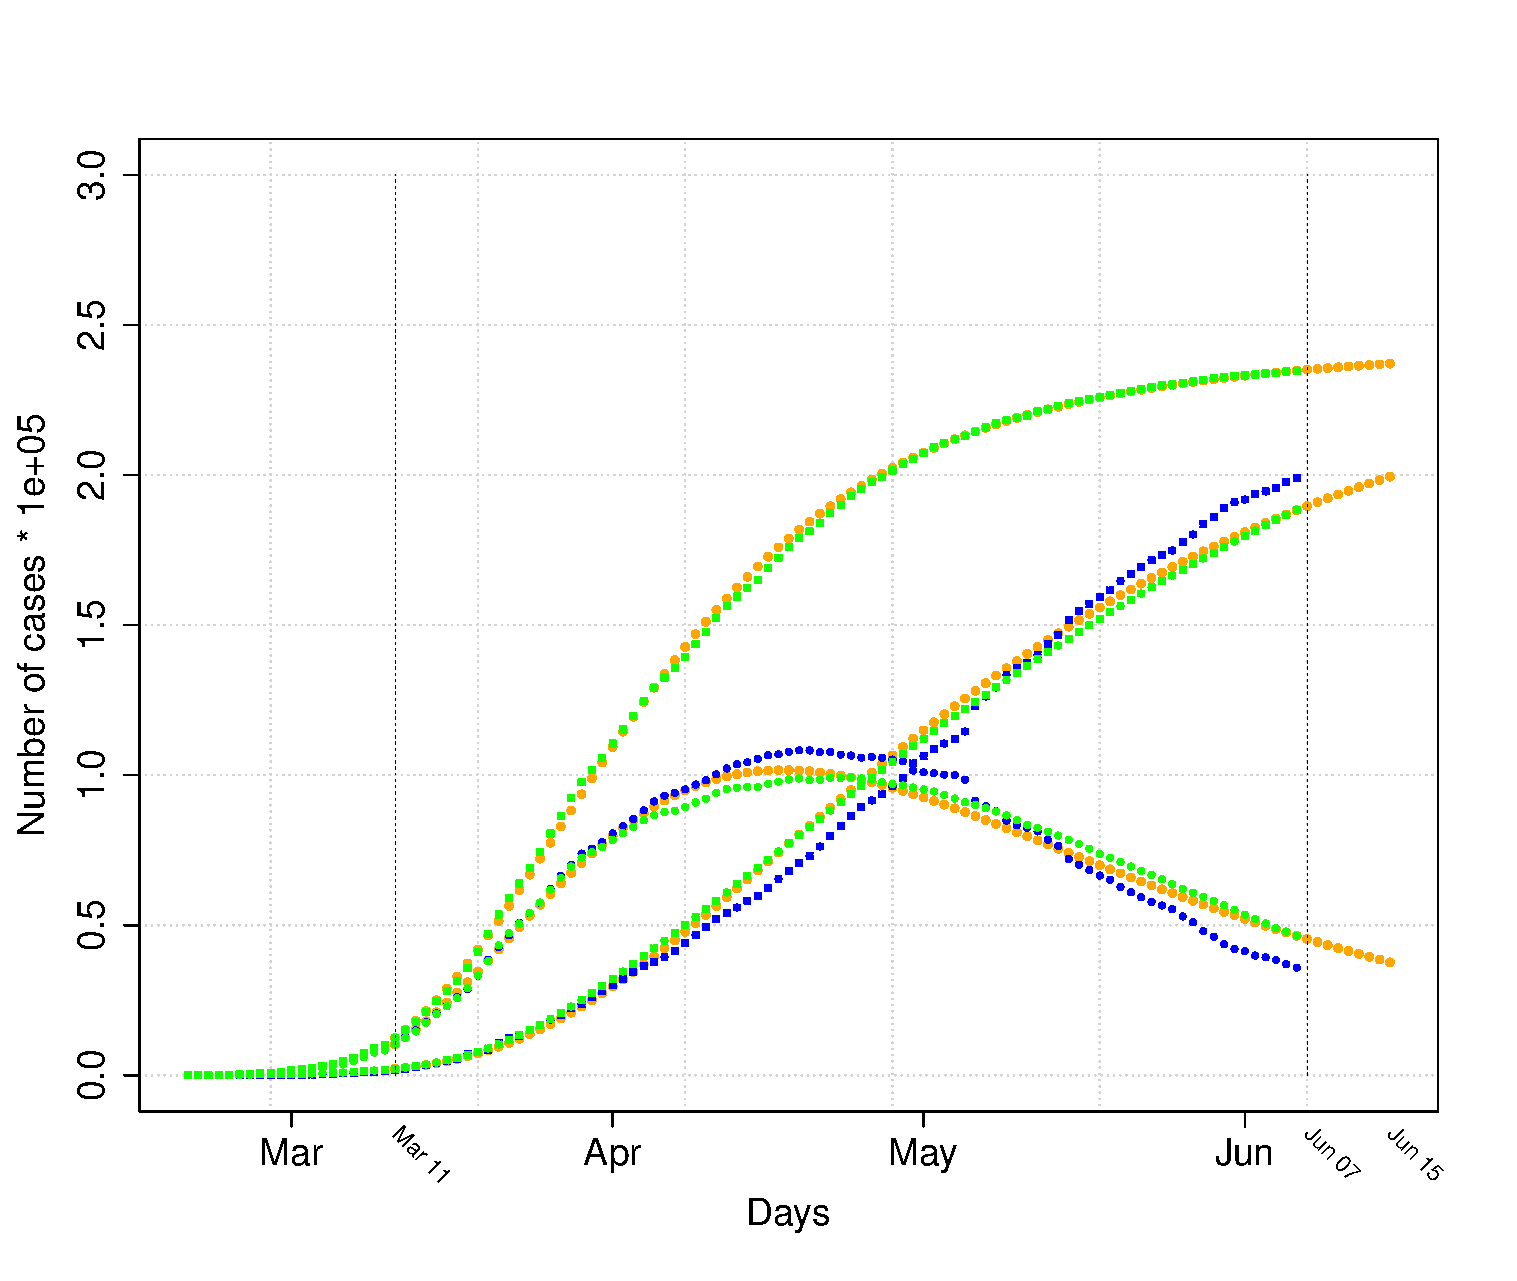
\includegraphics[width=2.5in,height=2in]{italy_figure_b_07_06_2020.eps}}
\end{center}
\begin{center}
\caption{SIR model, data pre-processing and RTT solution, Italy, March to June 2020
}
\label{fig:italy_sir_model_07_06_2020}
\end{center}
\end{figure}


\begin{figure}
\begin{center}
%\subfloat [Second-chance model and absolute standard normal]
{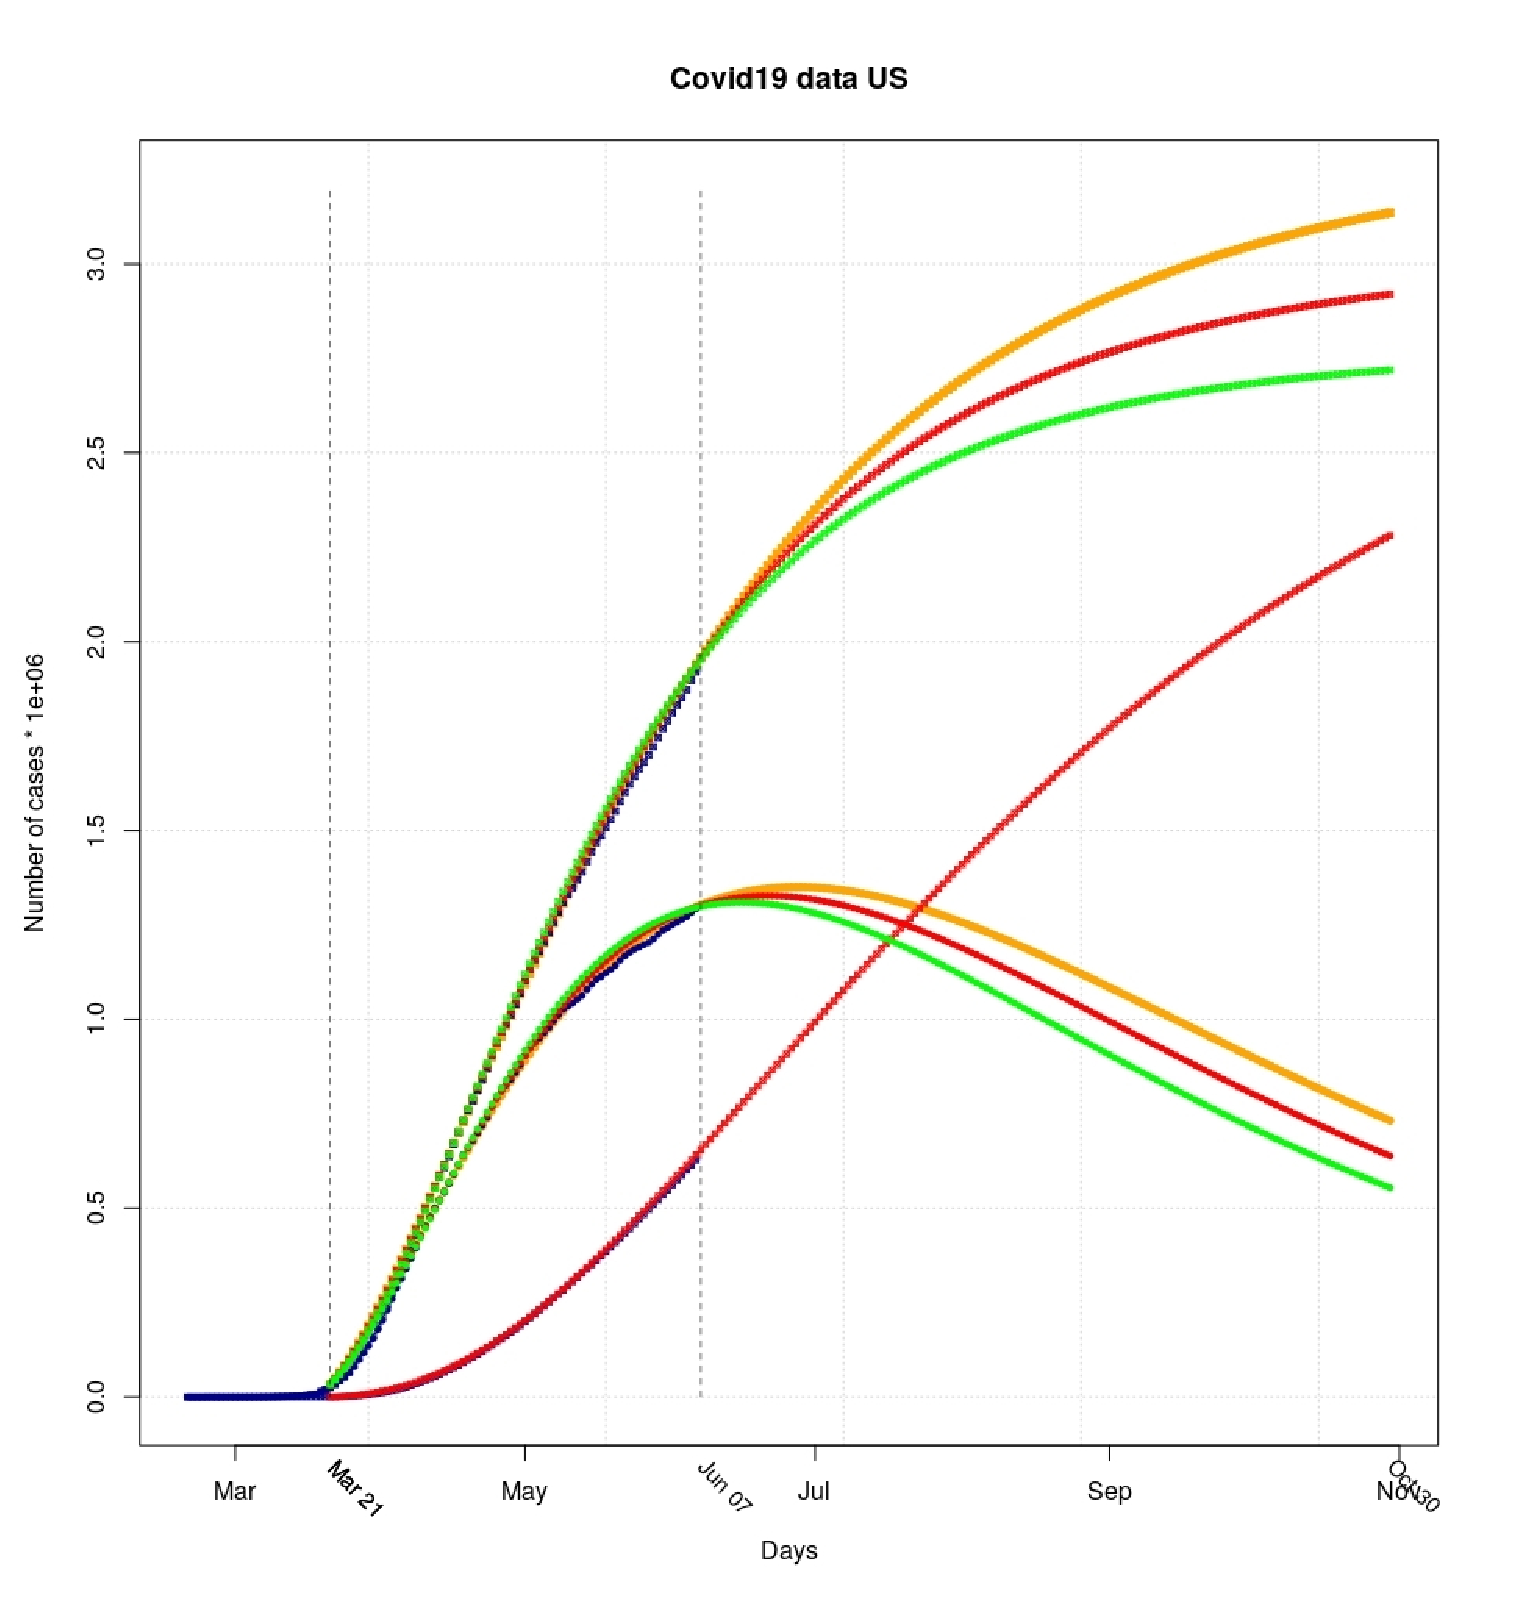
\includegraphics[width=2.5in,height=2in]{usa_figure_a_07_06_2020.eps}}
\qquad
{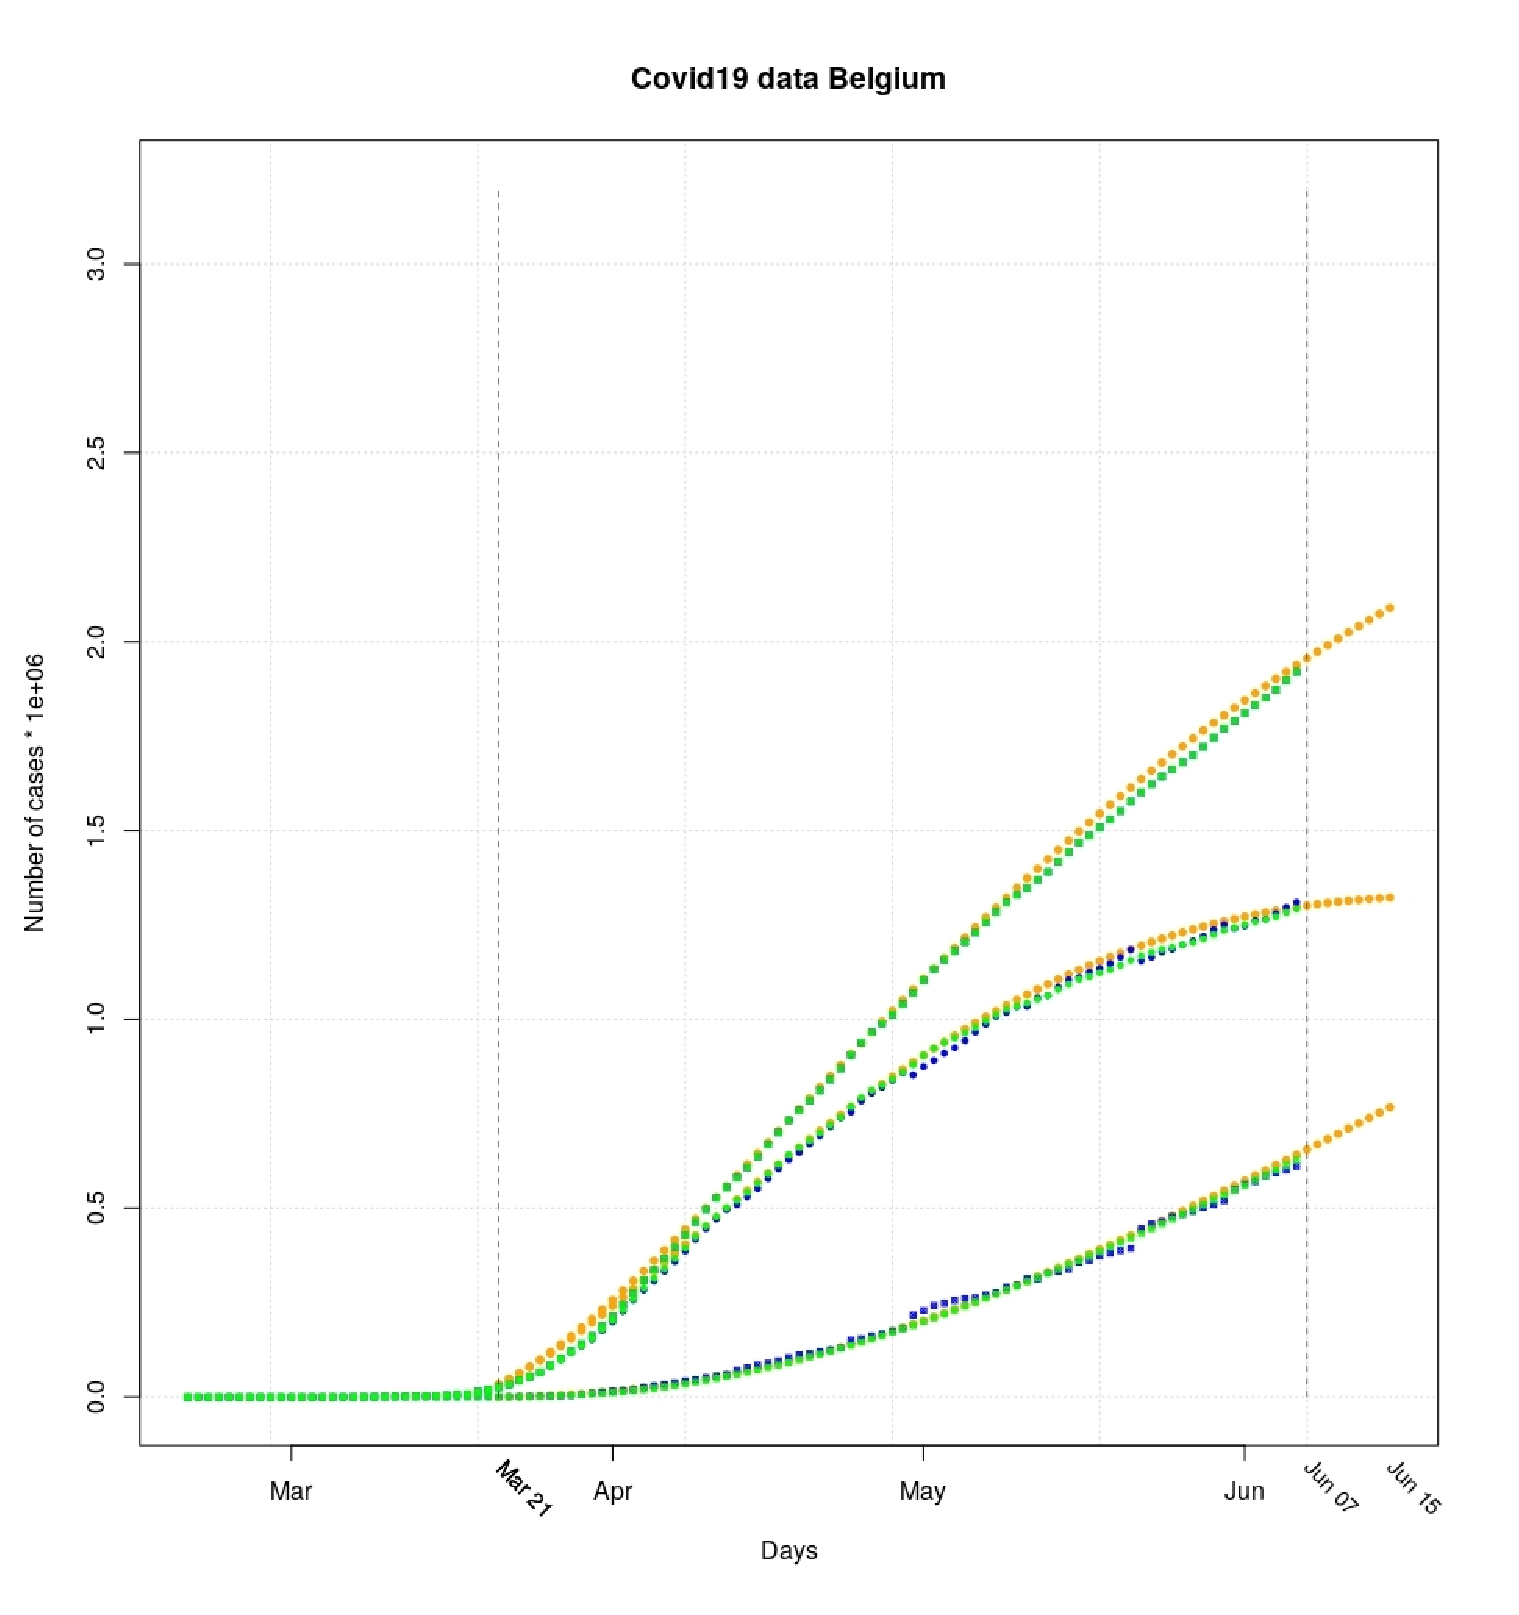
\includegraphics[width=2.5in,height=2in]{usa_figure_b_07_06_2020.eps}}
\end{center}
\begin{center}
\caption{SIR model, data pre-processing and RTT solution, USA, March to June 2020
}
\label{fig:usa_sir_model_07_06_2020}
\end{center}
\end{figure}

\newpage

\noindent The data of Italy and USA show close agreement between raw and pre-processed versions, with the pre-processed version smoothing relatively sharp jumps in the raw data.

\bigskip

\noindent The data of Brazil show close agreement, but still at an early stage in the epidemic.

\bigskip

\noindent Regression pre-processing as tool for reverse engineering. It has been announced that Belgium recorded as affected cases also those under doubt. As a result, it appears as if it holds record high deaths per million, and number of infected cases that is still growing on June 7th, unlike all its neighbors. Pre-processing is in sharp disagreement with the raw data, placing Belgium in the same standard stage as its neighbors, well past the transition to $R_0$ below $1$, and suggesting lethality not above standard European levels.

\bigskip

\noindent The data of Chile and France show drastic corrections in the number of recovered cases, rendering analysis difficult. Although Chilean raw and modified data show agreement when the last 10 days are omitted, the later drastic corrections place accuracy in doubt.

\bigskip

The data of Iran and Israel show clear evidence of exit from steady conditions. However, Israel pre-processed data show some disagreement with pre-processed data already before relaxing restrictions.

\newpage

\noindent {\bf The RTT method to solve differential equations with data subject to noise - Bassan, Marcus, Meilijson and Talpaz 1997}

\bigskip

\noindent Relatively novel theoretical contribution, RTT method to mimic ODE by stochastic counterparts, simpler but related to the SDE based on Diffusion processes via Fokker-Planck. Based on Skew-product transformations in Ergodic theory.

\bigskip

\noindent Diffusion methods place noise vertically, RTT method adopts the solution to the ODE, but considers it as evaluated at a random time process that advances on the average like chronological time. Thus, errors are horizontal.

\bigskip

\noindent Empirical data consist of $(X_1,R_1), (X_2,R_2), \dots, (X_n, R_n)$, from which the infected case totals \linebreak $Y_j=X_j-R_j$ can be inferred and then regre3ssion-modified if needed. The sequences $X$ and $R$ are assumed or forced to be non-decreasing.

\bigskip

\noindent No attempt will be made to solve SIR analytically. Instead, a small increment of time $\delta={1 \over M}$ is set (say, $M=100$), and the ODE is solved numerically as a difference equation. 

\newpage

\noindent Fix $\beta, \gamma, K$ and the function $g$, initiate functions $x$ and $r$ as $X_1$ and $R_1$ respectively, initiate $i$ as $X_1-R_1$ and proceed with the definition for $j \ge 2$
\begin{eqnarray}
x(j)&=&x(j-1)+\beta g(i(j-1))(1-{{x(j-1)} \over K}) \delta \nonumber \\
r(j)&=&r(j-1)+\gamma i(j-1) \delta \nonumber \\
i(j)&=&x(j)-r(j) \label{thesolution}
\end{eqnarray}

\bigskip

\noindent Define the {\em random time trajectory} as starting at $T_1(1)=1, T_2(1)=1$. 

\bigskip

\noindent For $m \ge 2$, let $T_1(m)$ be the smallest ${j \over M}$ for which $x(j) \ge X_j$ and let $T_2(m)$ be the smallest ${j \over M}$ for which $r(j) \ge R_j$.

\bigskip

\noindent Better yet, let $T_1(m)$ and $T_2(m)$ be the linear interpolants between $j-1$ and $j$ that achieve the values $X_m$ and $R_m$ exactly.

\bigskip

\noindent Now solve for $\beta$ and $\gamma$ so that $T_1(n)=T_2(n)=n$. Incremental time has average $1$ in both equations. 

\bigskip

\noindent Define $\Delta_1(m)=T_1(m+1)-T_1(m)$ and $\Delta_2(m)=T_2(m+1)-T_2(m)$, for $m=1, 2, \cdots,m-1$ as the (mean-$1$) increments of the $T_1$ amd $T_2$ processes.

\newpage

\noindent {\bf The likelihood function induced by the RTT method}. 

\bigskip

\noindent View the incremental times $(\Delta_1(m),\Delta_2(m))$ as observations from a bivariate mean-zero Gaussian distribution, and let $\Sigma$ be their empirical covariance matrix. Up to a multiplicative constant, the normal density evaluated at these data is $(\det(\Sigma))^{-{{n-1} \over 2}}$.

\bigskip

\noindent Alternatively, view the processes $T_1(m)-m$ and $T_2(m)-m$ as bivariate Gaussian random walk bridges.
These two models yield equivalent Gaussian density functions. As a result, the simpler as-if i.i.d. formulation is adopted. 

\bigskip

\noindent Perhaps a better stochastic model would be to let $(\Delta_1(m),\Delta_2(m))$ be first passage times of constant heights by BM. Density is well known. In this context, the RTT method is similar to SDE with diffusion term proportional to the drift term. Details are skipped but included below.

\bigskip

\noindent The random time likelihood function for the RTT model is obtained by multiplying the random time density above by the Jacobian of the transformation, the ratio $1$ over the product over the sample of the differential terms $\beta g(X_m-R_m)(1-X_m/K)$ and $\gamma (X_m-R_m)$.

\bigskip

\noindent $K$ and $\alpha$ are MLE-estimated by maximizing the logarithm of the profile likelihood function, and their standard errors (and correlation coefficient, if needed) are estimated as usual, via the empirical Fisher information.

\newpage

\begin{table}
\begin{center}
\begin{tabular}{l|ccccccc|r}
Country & $\alpha$ & $\beta$ & $\gamma$ & $\sigma_X $ & $ \sigma_R$ & $\rho$ & $K$ & $X_{max}$ \\ \hline
Belgium & $0.497$ & $16.06$ & $0.014$ & $0.296$ & $0.071$ & $0.240$ & $61510$ & $59072$ \\
Brazil  & $0.849$ & $0.57$ & $0.046$ & $0.255$ & $0.148$ & $0.578$ & N/A & $672846$ \\
%Chile   & 0.48 & 1.2318 &0.0450 &  55 &  113 & 50 & 0.9897 &  \\
%France  & 0.91 & 0.0025 &  0.0278& 38 & 72 & 1 & 0.9973 &  \\
Germany & $0.382$ & $131.00$ & $0.070$ & $0.343$ & $0.044$ & $0.127$ & $198917$ & $185450$ \\
%Israel & 0.01 &  292.61 & 0.0379 & 57 &  84& 59 & 0.9870 & \\
Italy  & $0.605$ & $9.97$ & $0.030$ & $0.193$ & $0.079$ & $0.410$ & $246234$ & $234801$ \\
Switzerland & 0.586	 &	10.8 & 0.067 & 0.228  & 0.535 & 0.252 & 31575&      30956	    \\
USA    & $0.246$  & $1380.26$ & $0.011$ & $0.118$ & $0.023$ & $0.192$ & $3370399$ & $1920061$ \\ \hline
\end{tabular}
\caption{
Parameter estimation based on data until June 7, 2020
\label{tablejune7}
}
\end{center}
\end{table}

\bigskip

\begin{table}
\begin{center}
\begin{tabular}{l|ccccccc|r}
Country & $\alpha$ & $\beta$ & $\gamma$ & $\sigma_X $ & $ \sigma_R$ & $\rho$ & $K$ & $X_{max}$ \\ \hline
Italy  & $0.605$ & $9.99$ & $0.028$ & $0.168$ & $0.063$ & $0.377$ & $245431$ & $230158$ \\
USA    & $0.272$  & $478.24$ & $0.011$ & $0.143$ & $0.042$ & $0.294$ & $2699321$ & $1662302$\\ \hline
\end{tabular}
\caption{
Parameter estimation based on data until May 25, 2020
\label{tablemay25}
}
\end{center}
\end{table}


\begin{figure}
\begin{center}
%\subfloat [Second-chance model and absolute standard normal]
{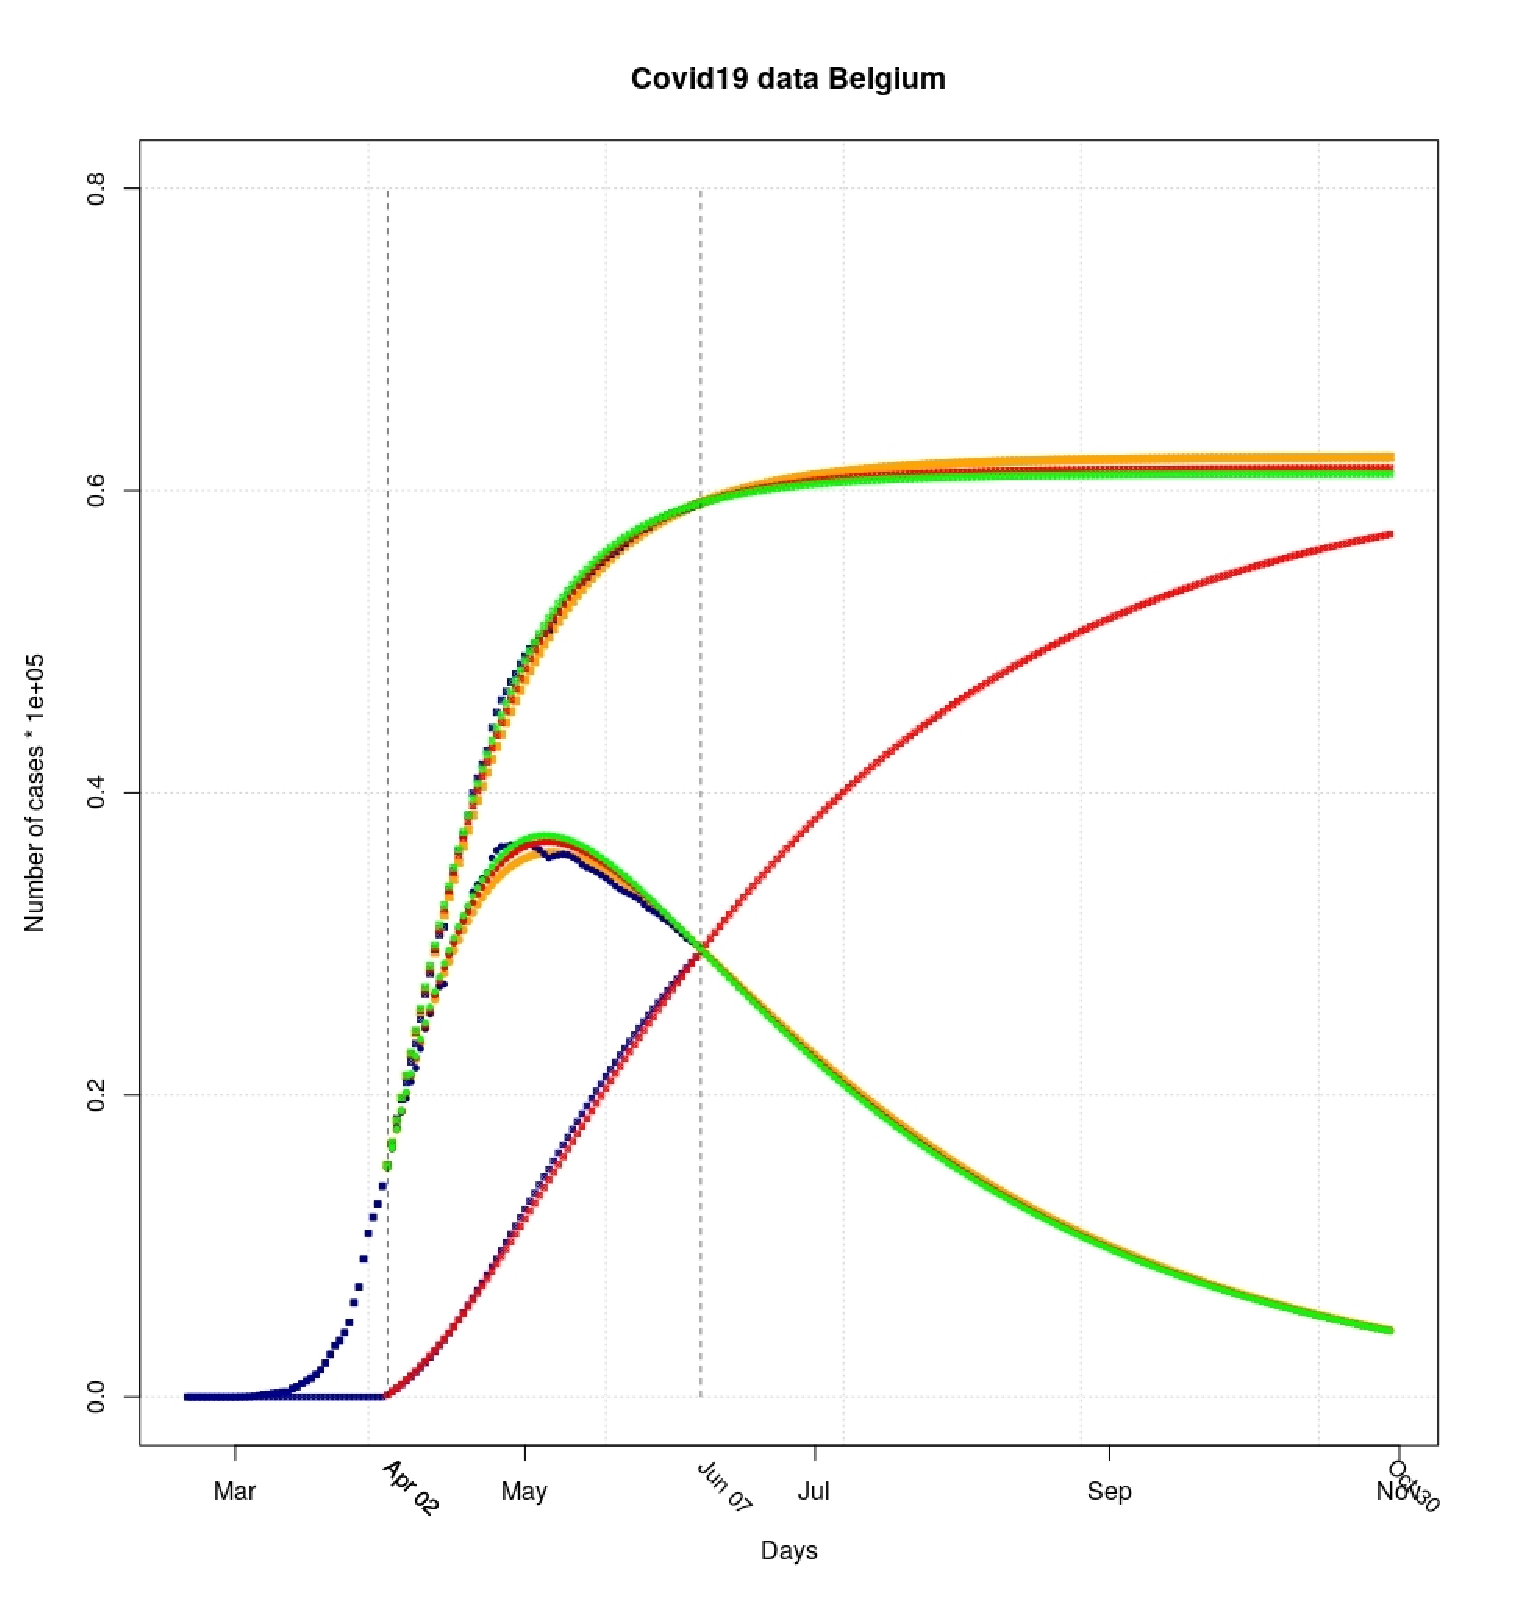
\includegraphics[width=2.5in,height=2in]{belgium_figure_a_07_06_2020.eps}}
\qquad
{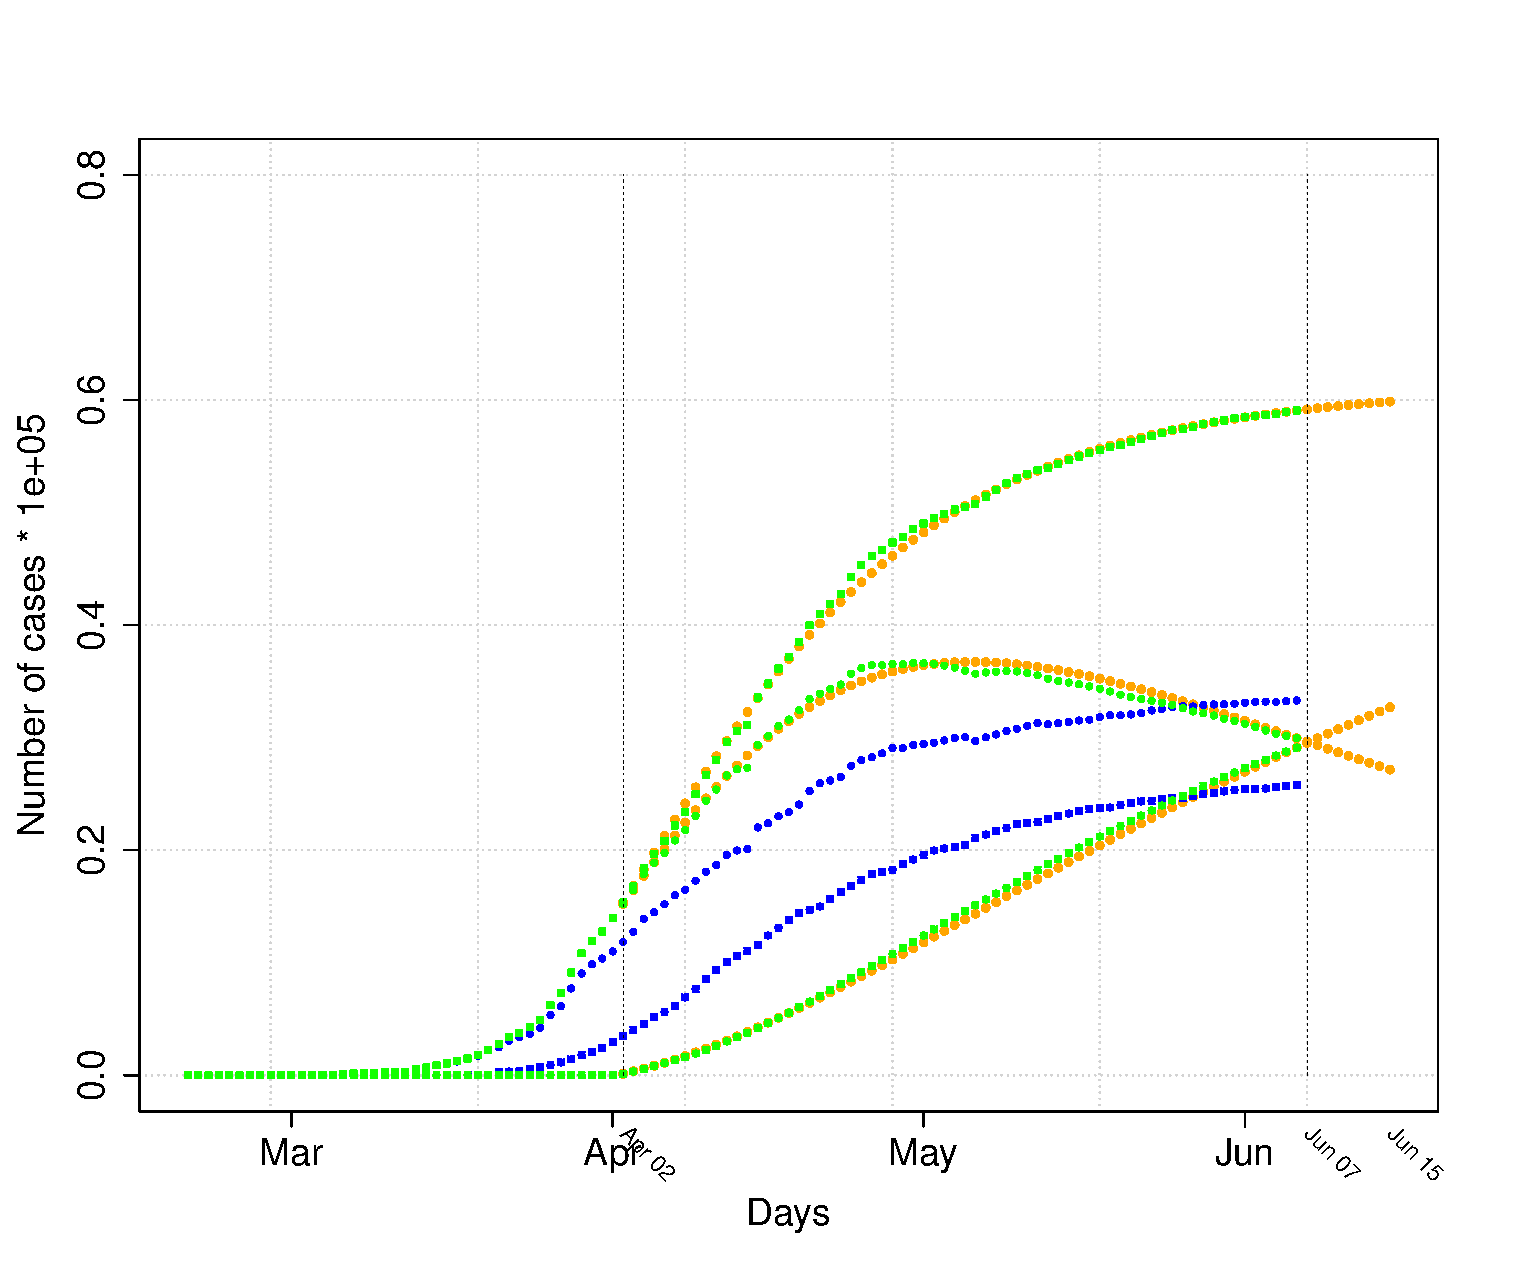
\includegraphics[width=2.5in,height=2in]{belgium_figure_b_07_06_2020.eps}}
\end{center}
\begin{center}
\caption{SIR model, data pre-processing and RTT solution, Belgium, March to June 2020
}
\label{fig:belgium_sir_model_07_06_2020}
\end{center}
\end{figure}

\begin{figure}
\begin{center}
%\subfloat [Second-chance model and absolute standard normal]
{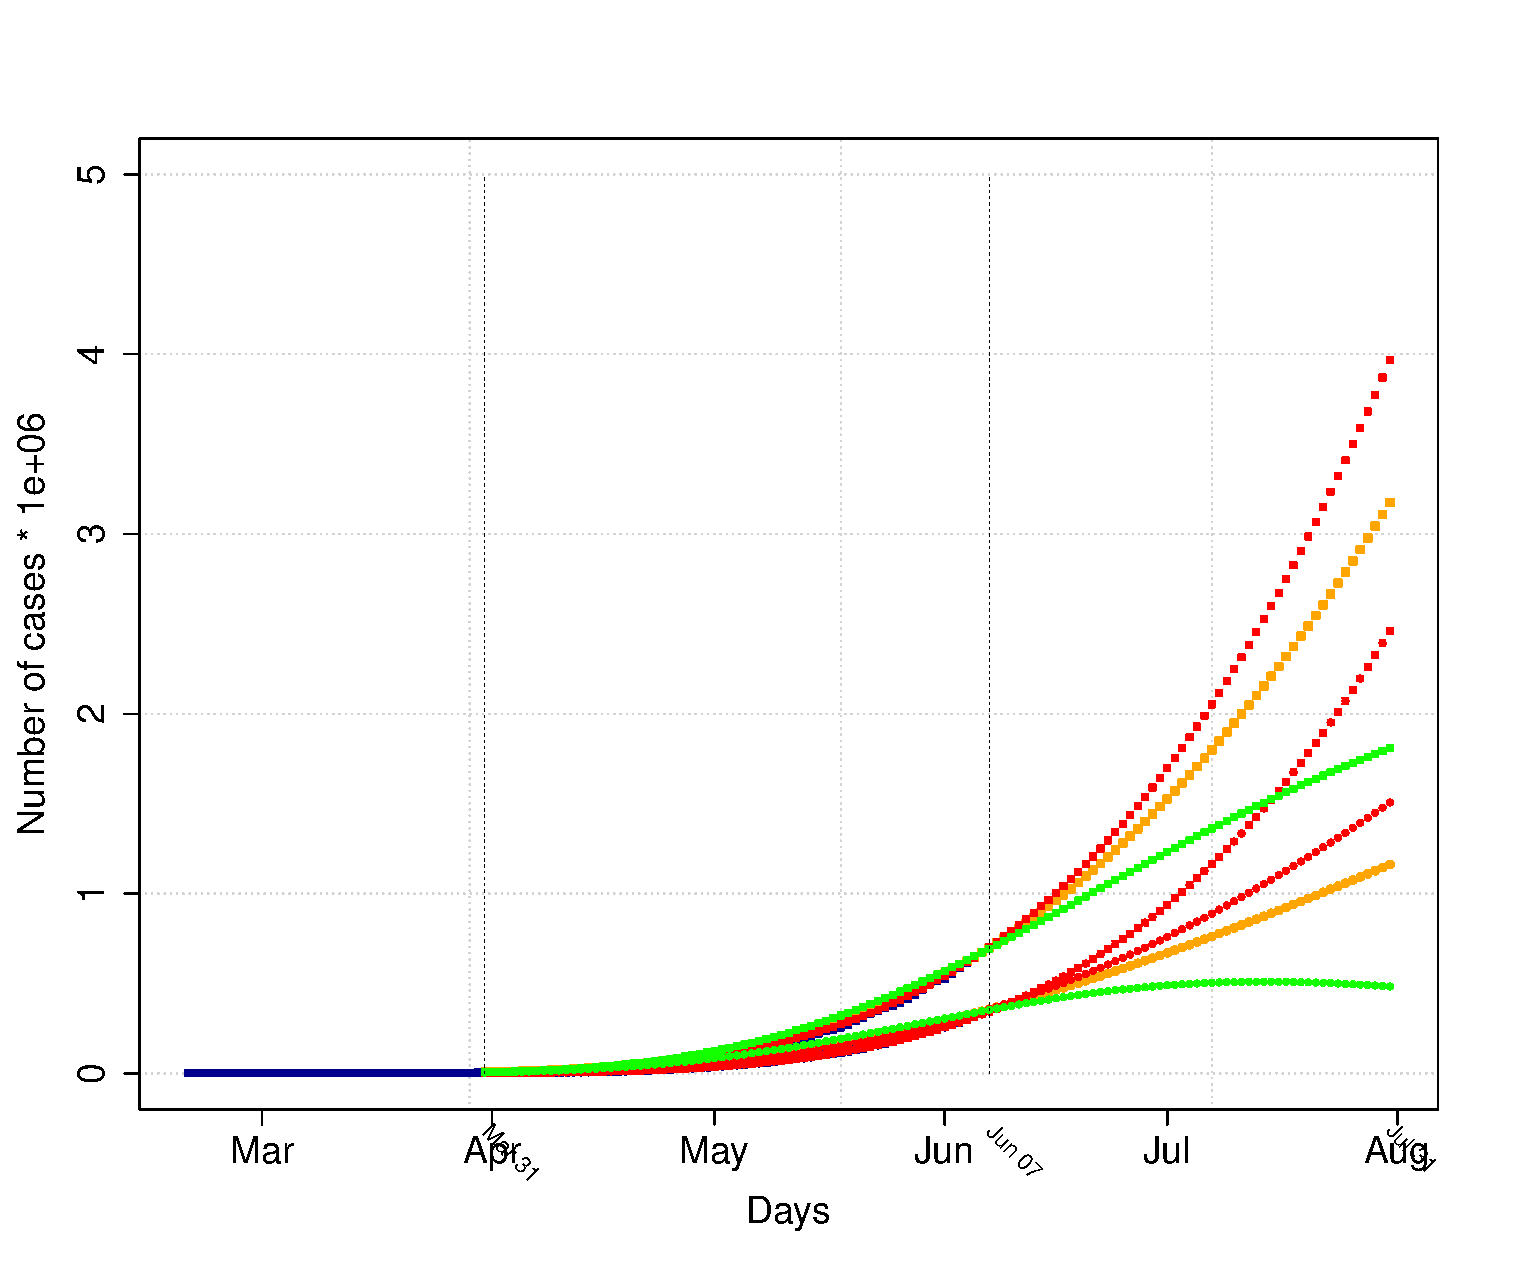
\includegraphics[width=2.5in,height=2in]{brazil_figure_a_07_06_2020.eps}}
\qquad
{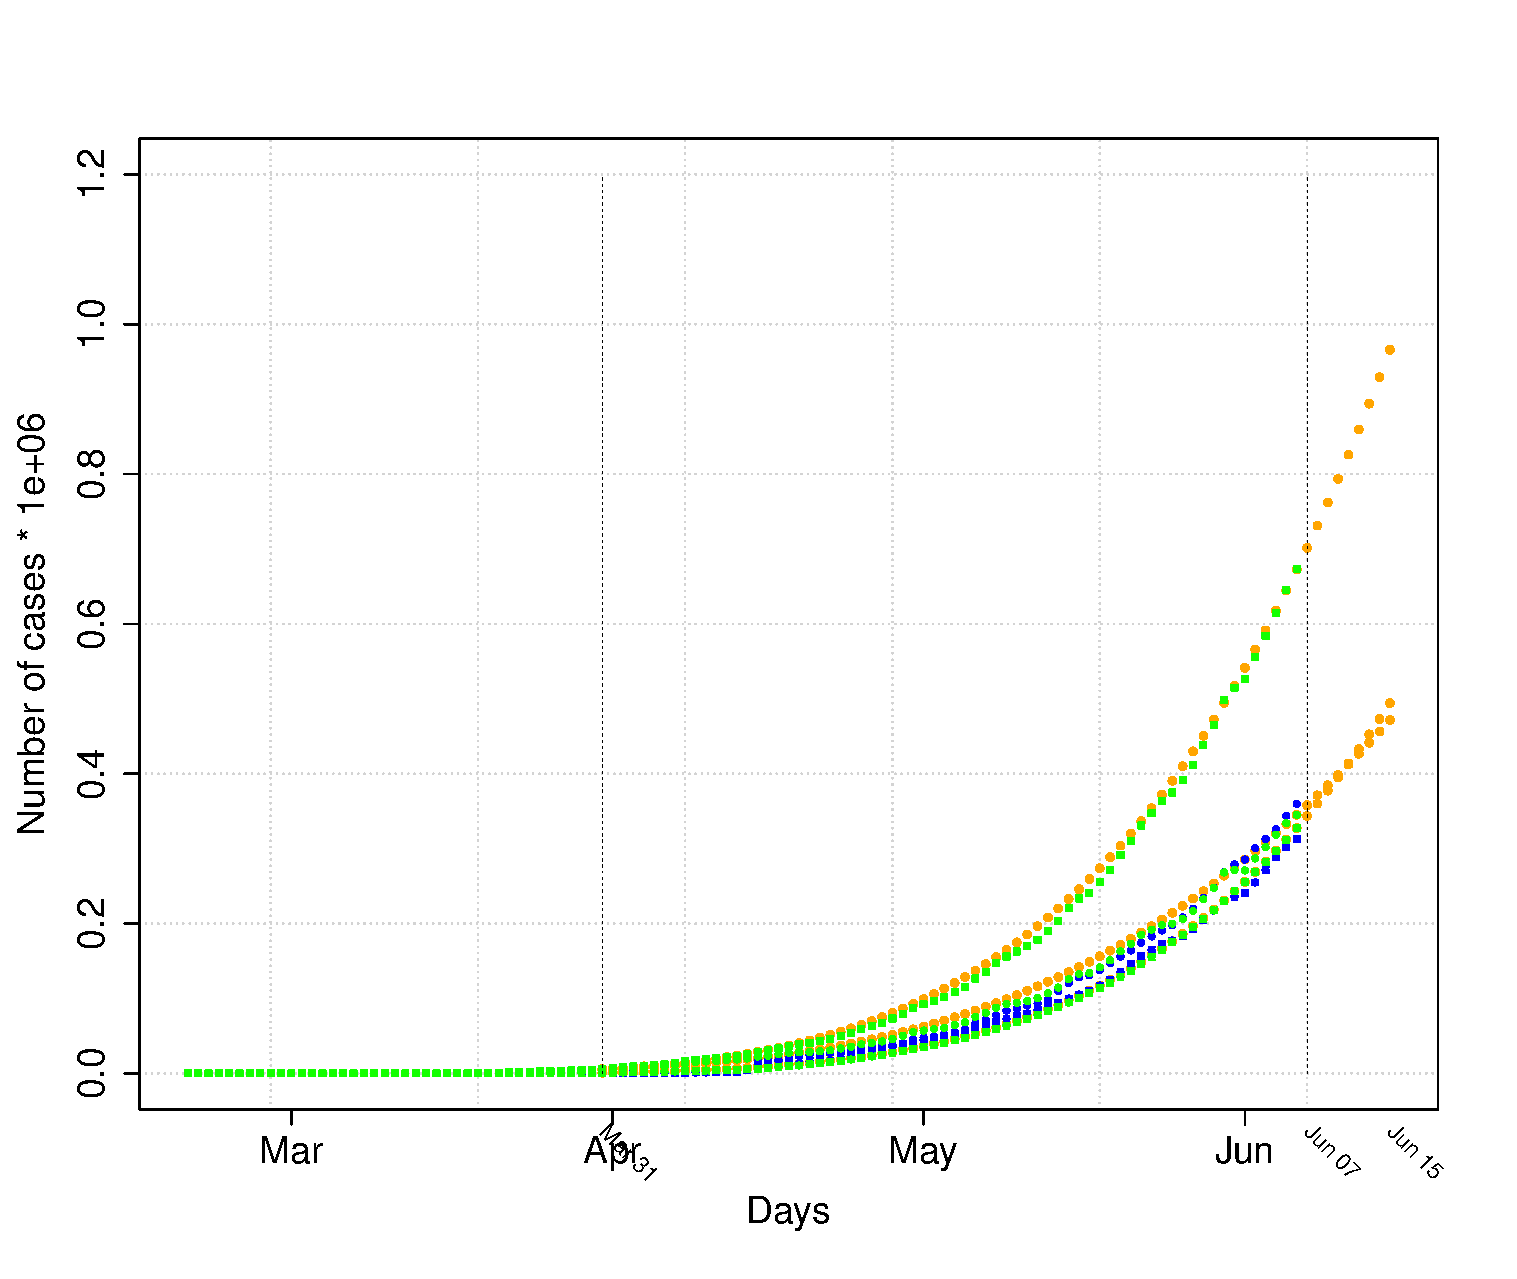
\includegraphics[width=2.5in,height=2in]{brazil_figure_b_07_06_2020.eps}}
\end{center}
\begin{center}
\caption{SIR model, data pre-processing and RTT solution, Brazil, March to June 2020
}
\label{fig:brazil_sir_model_07_06_2020}
\end{center}
\end{figure}

\begin{figure}
\begin{center}
%\subfloat [Second-chance model and absolute standard normal]
{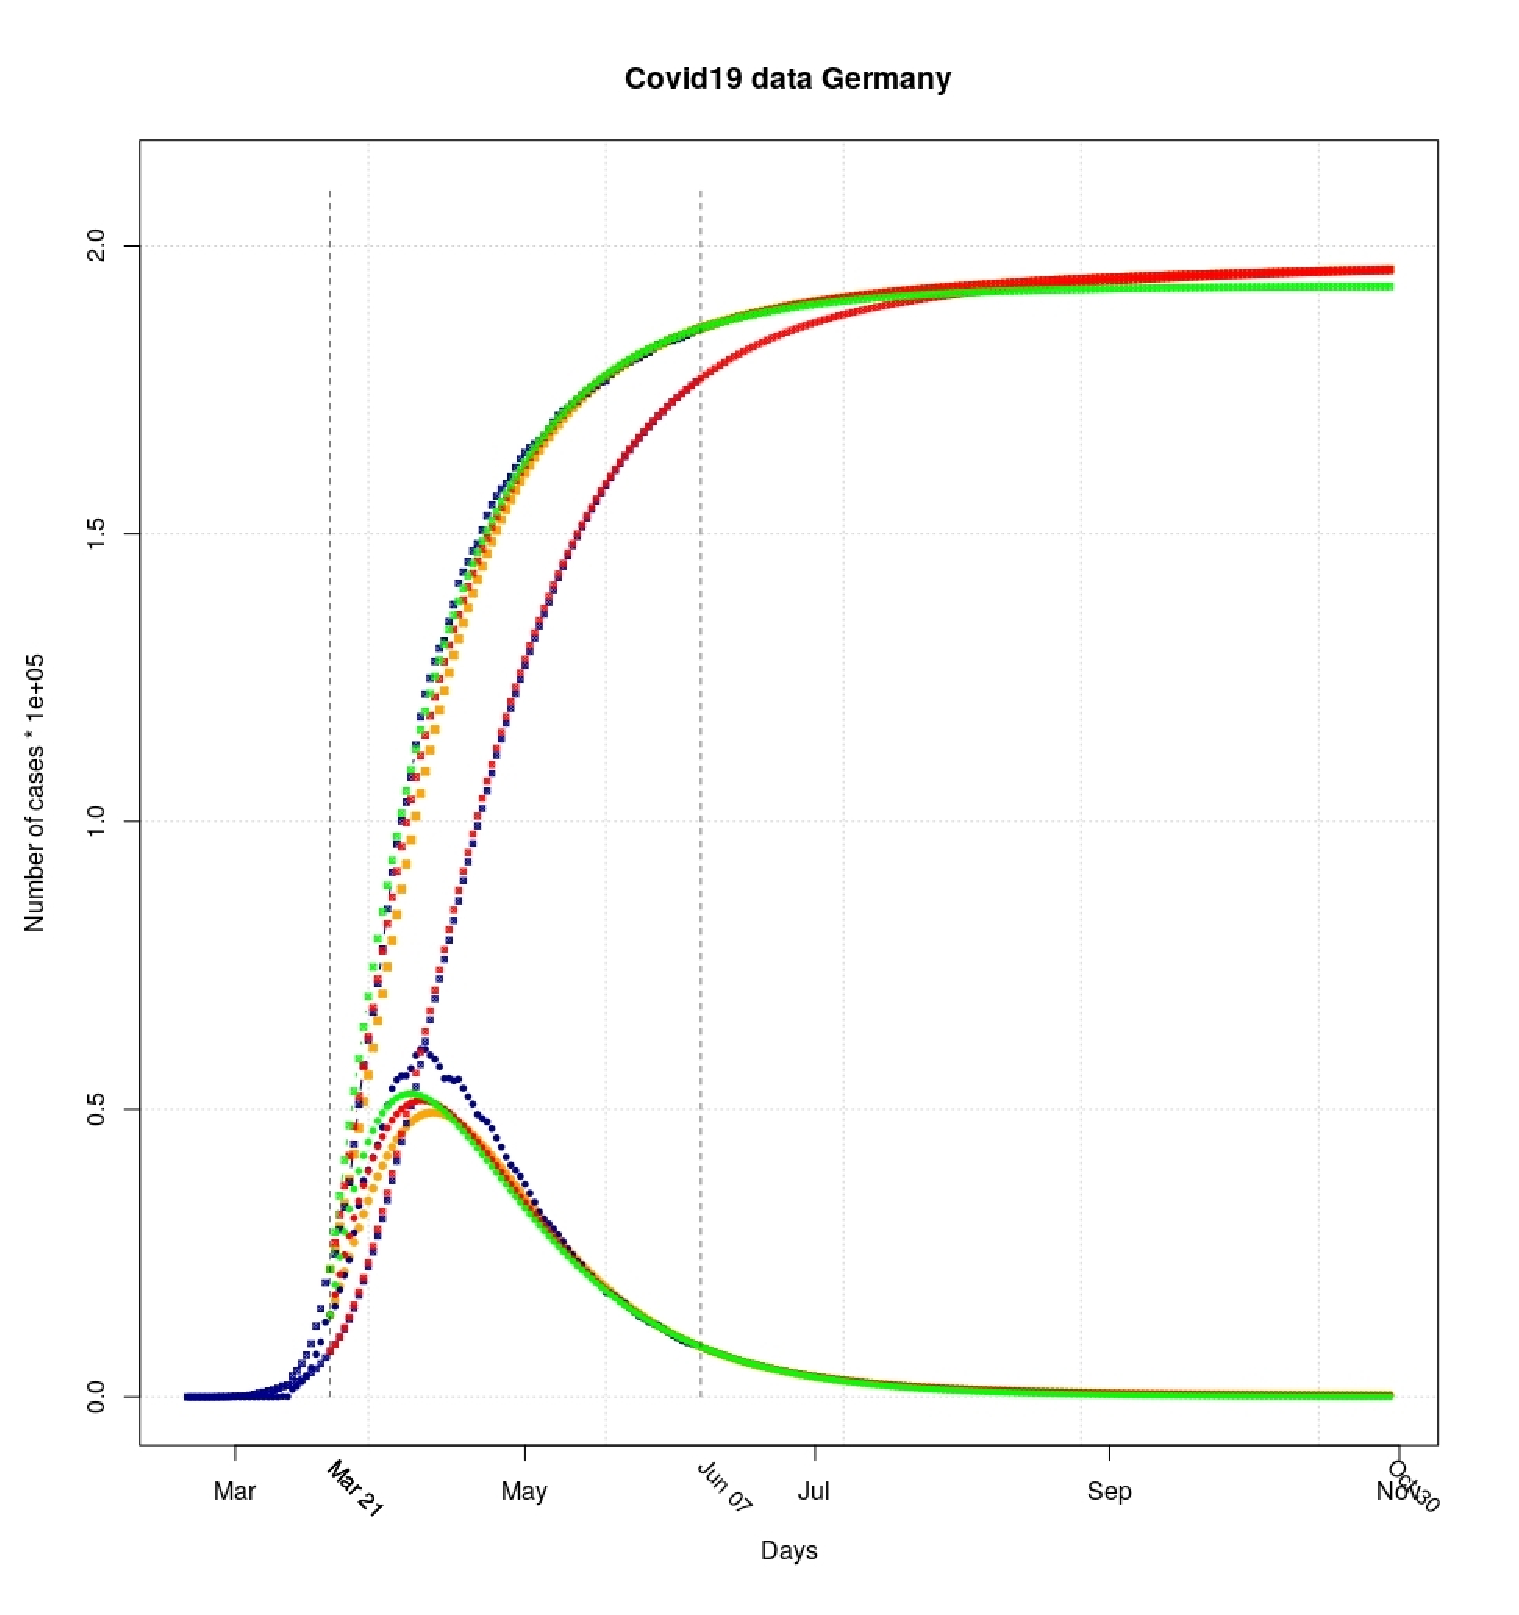
\includegraphics[width=2.5in,height=2in]{germany_figure_a_07_06_2020.eps}}
\qquad
{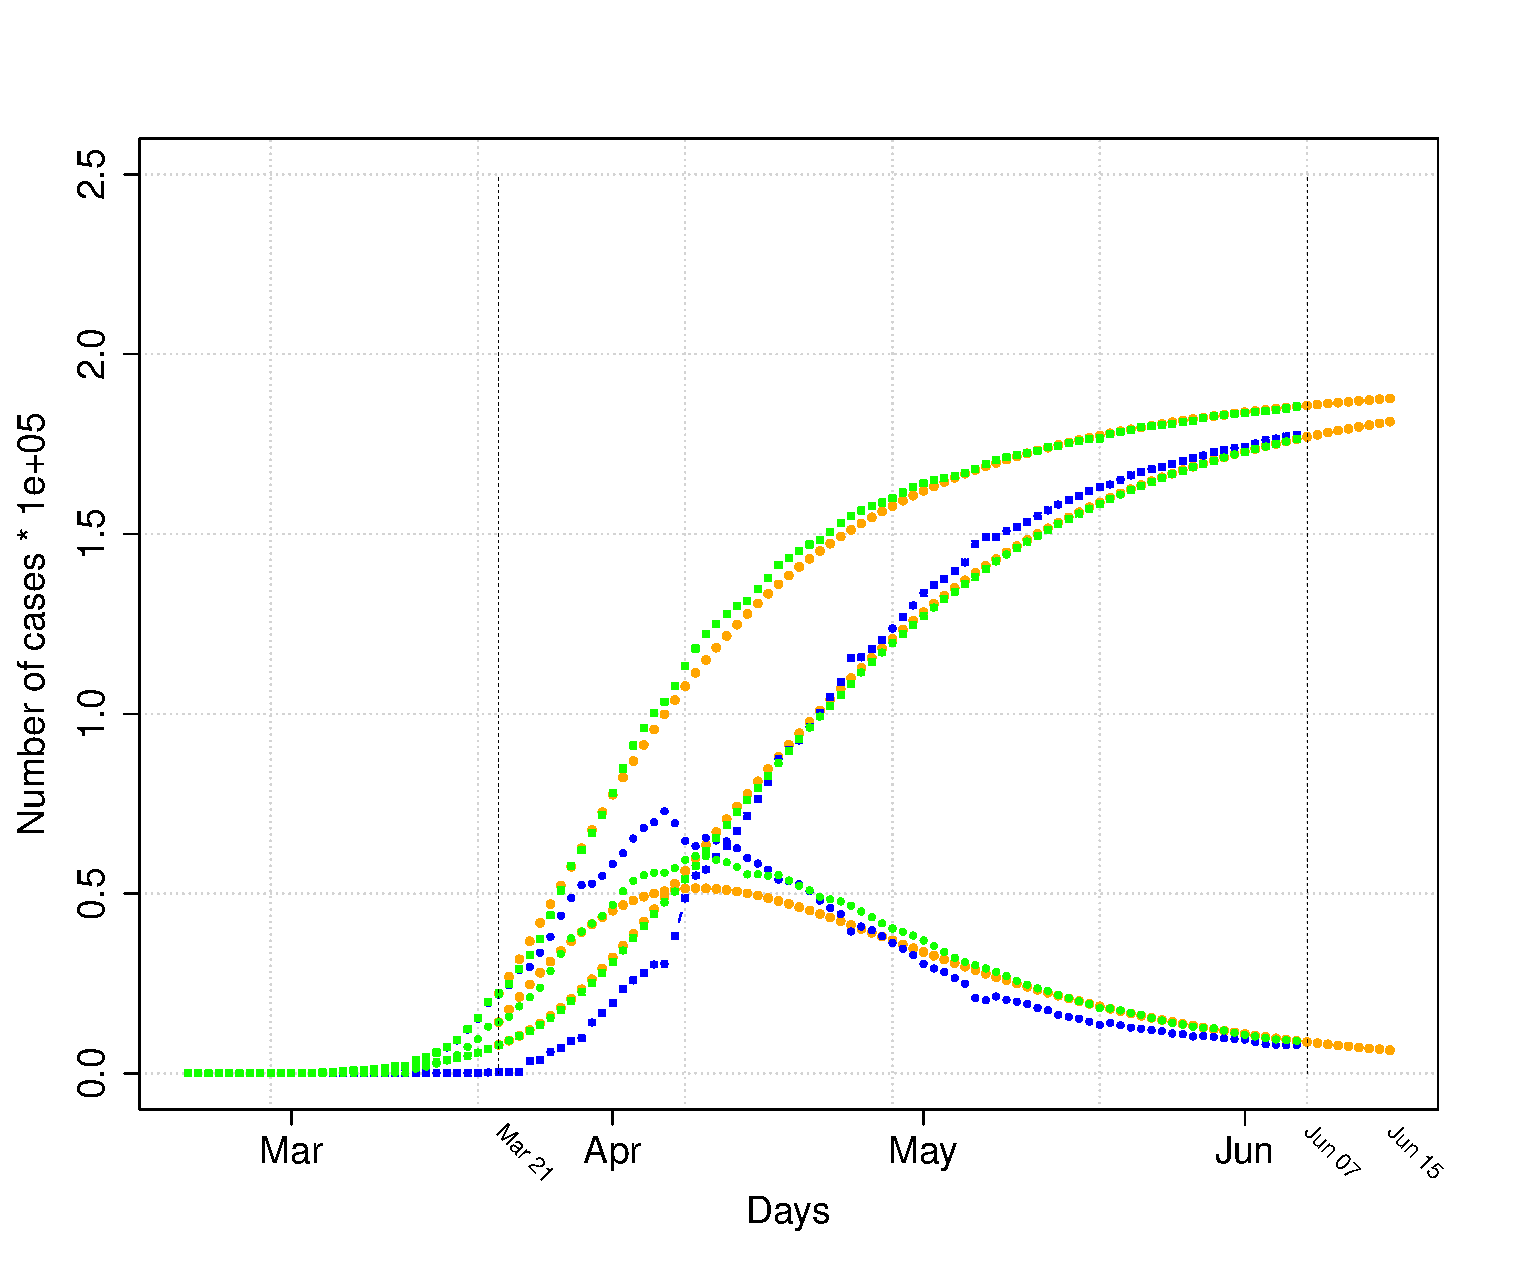
\includegraphics[width=2.5in,height=2in]{germany_figure_b_07_06_2020.eps}}
\end{center}
\begin{center}
\caption{SIR model, data pre-processing and RTT solution, Germany, March to June 2020
}
\label{fig:germany_sir_model_07_06_2020}
\end{center}
\end{figure}

\begin{figure}
\begin{center}
%\subfloat [Second-chance model and absolute standard normal]
{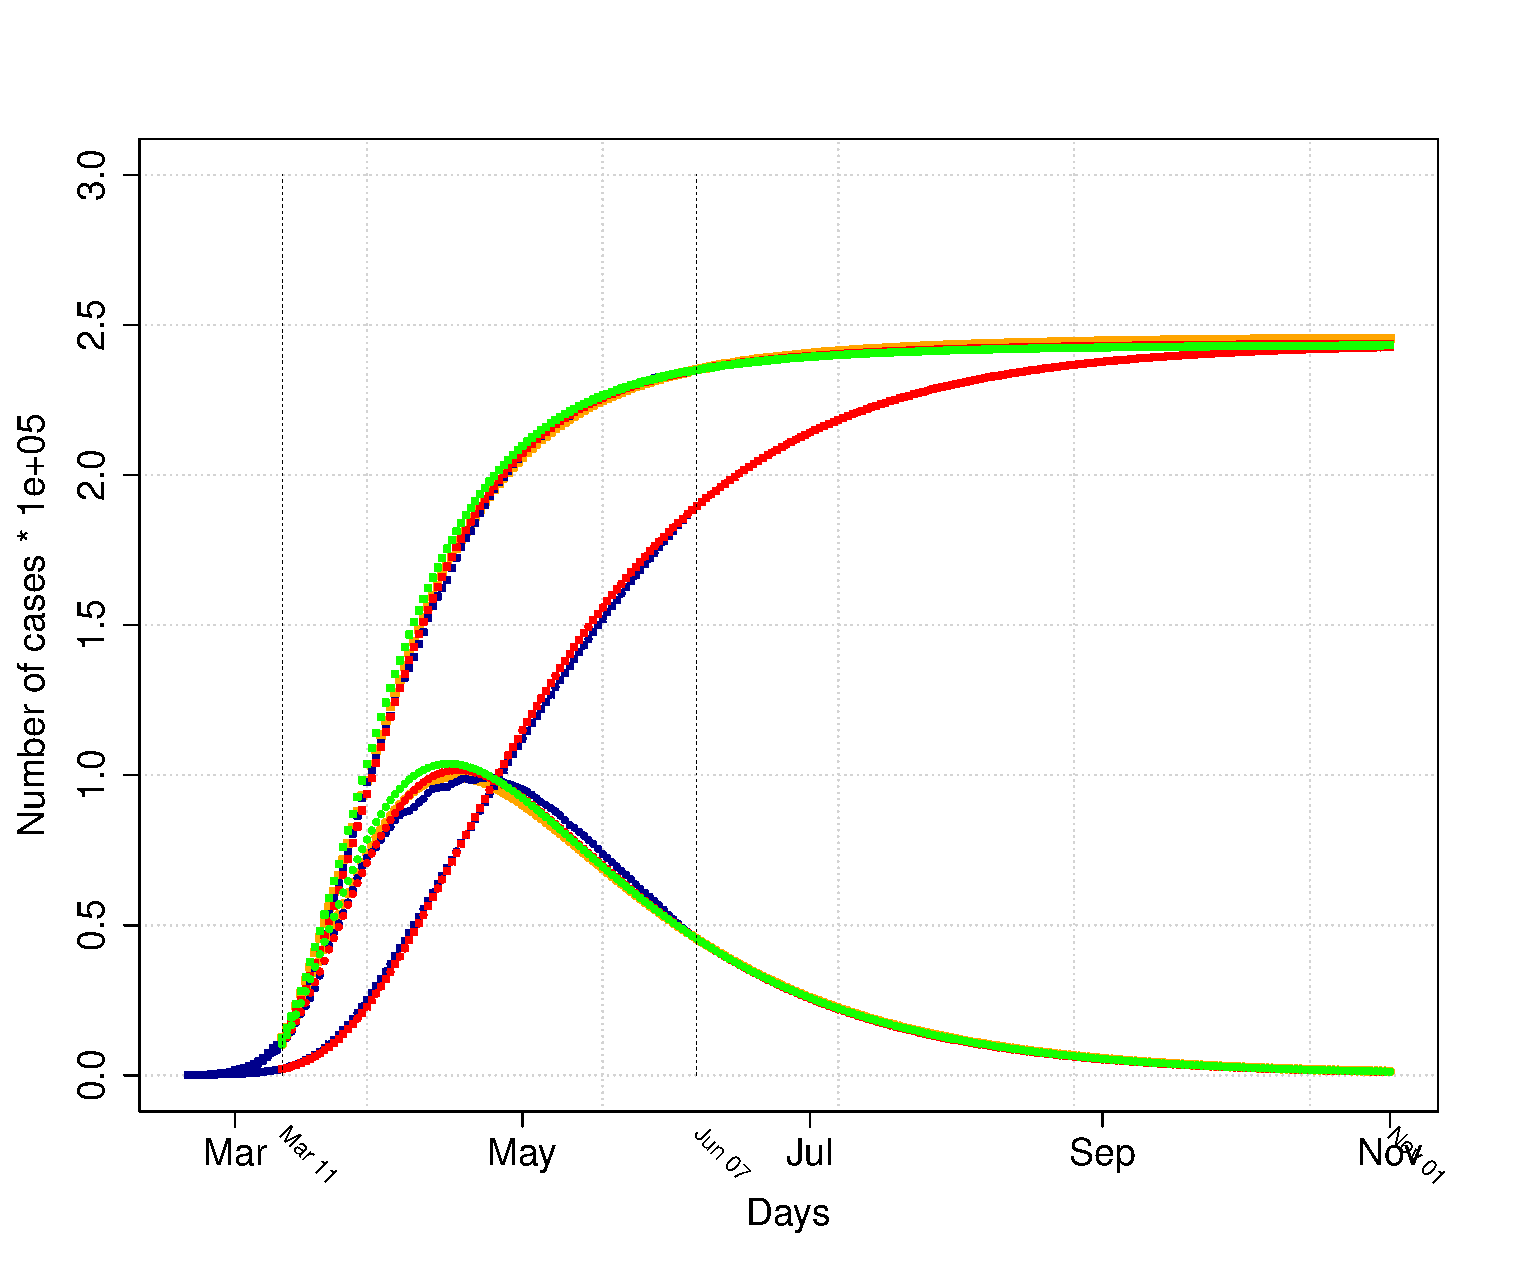
\includegraphics[width=2.5in,height=2in]{italy_figure_a_07_06_2020.eps}}
\qquad
{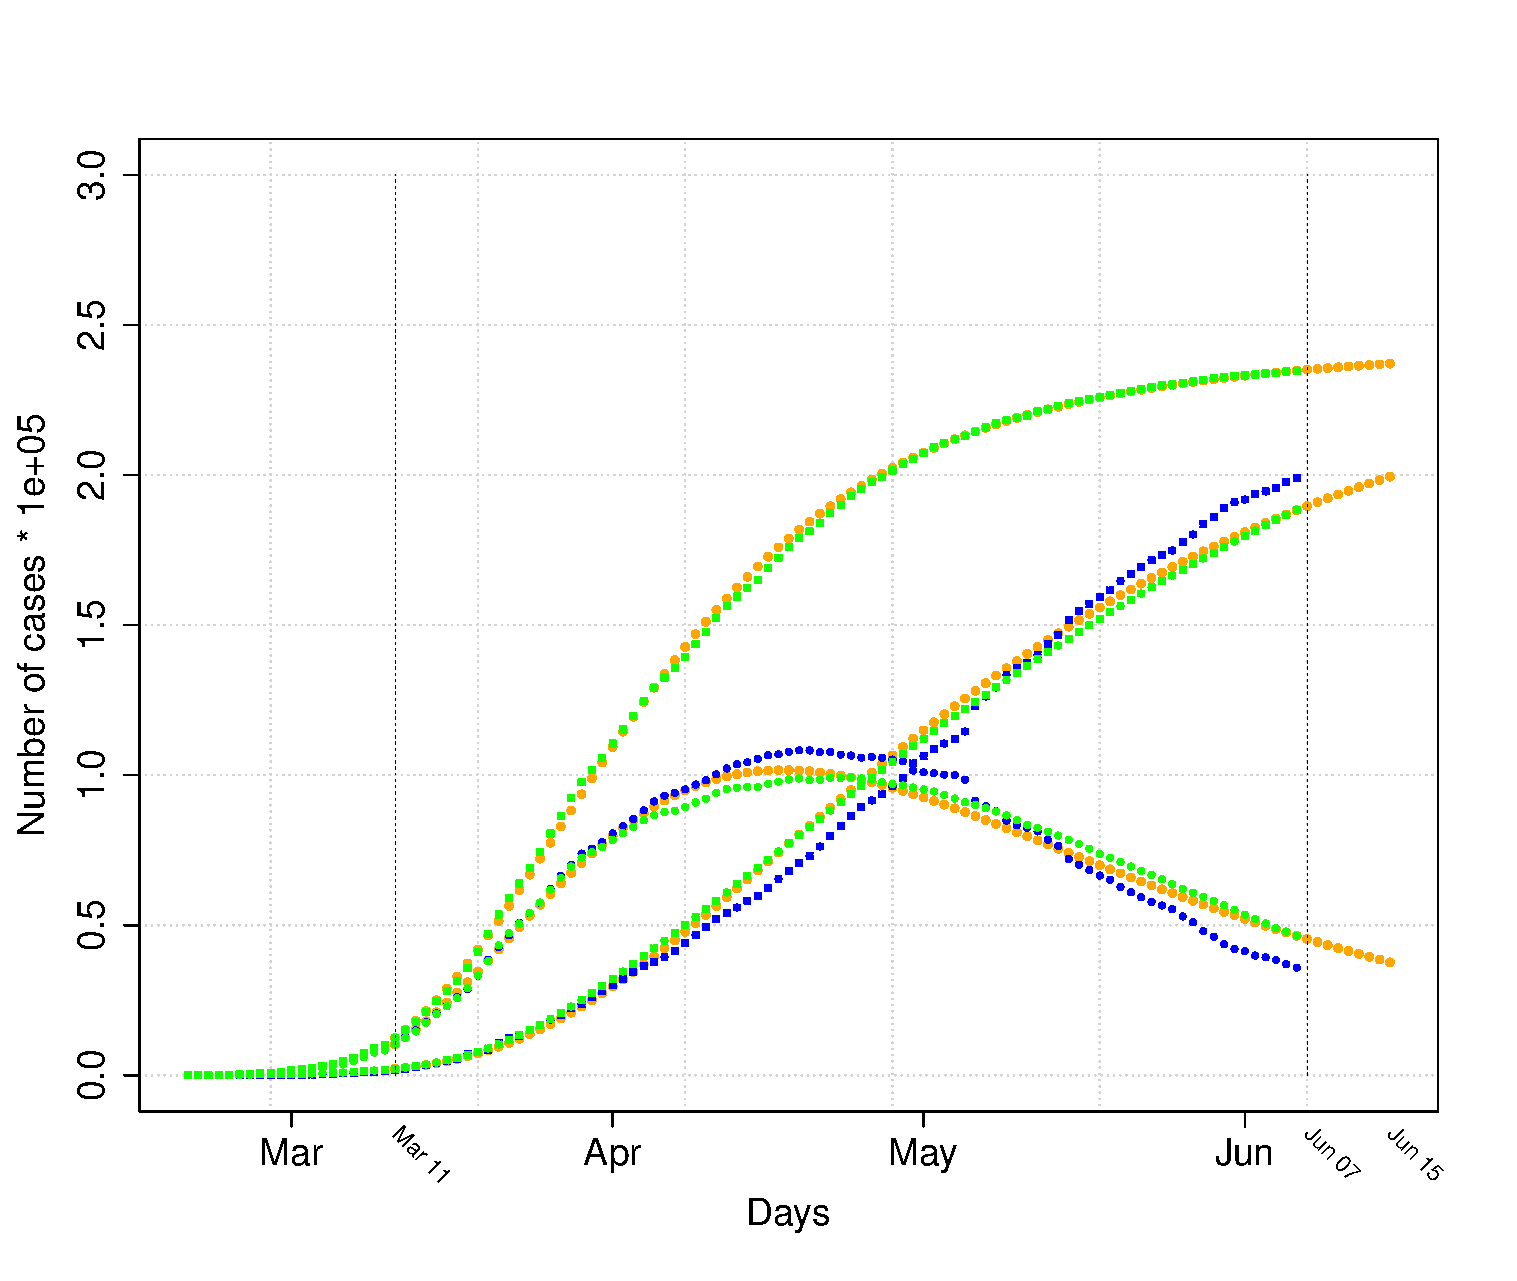
\includegraphics[width=2.5in,height=2in]{italy_figure_b_07_06_2020.eps}}
\end{center}
\begin{center}
\caption{SIR model, data pre-processing and RTT solution, Italy, March to June 2020
}
\label{fig:italy_sir_model_07_06_2020}
\end{center}
\end{figure}

\begin{figure}
\begin{center}
%\subfloat [Second-chance model and absolute standard normal]
{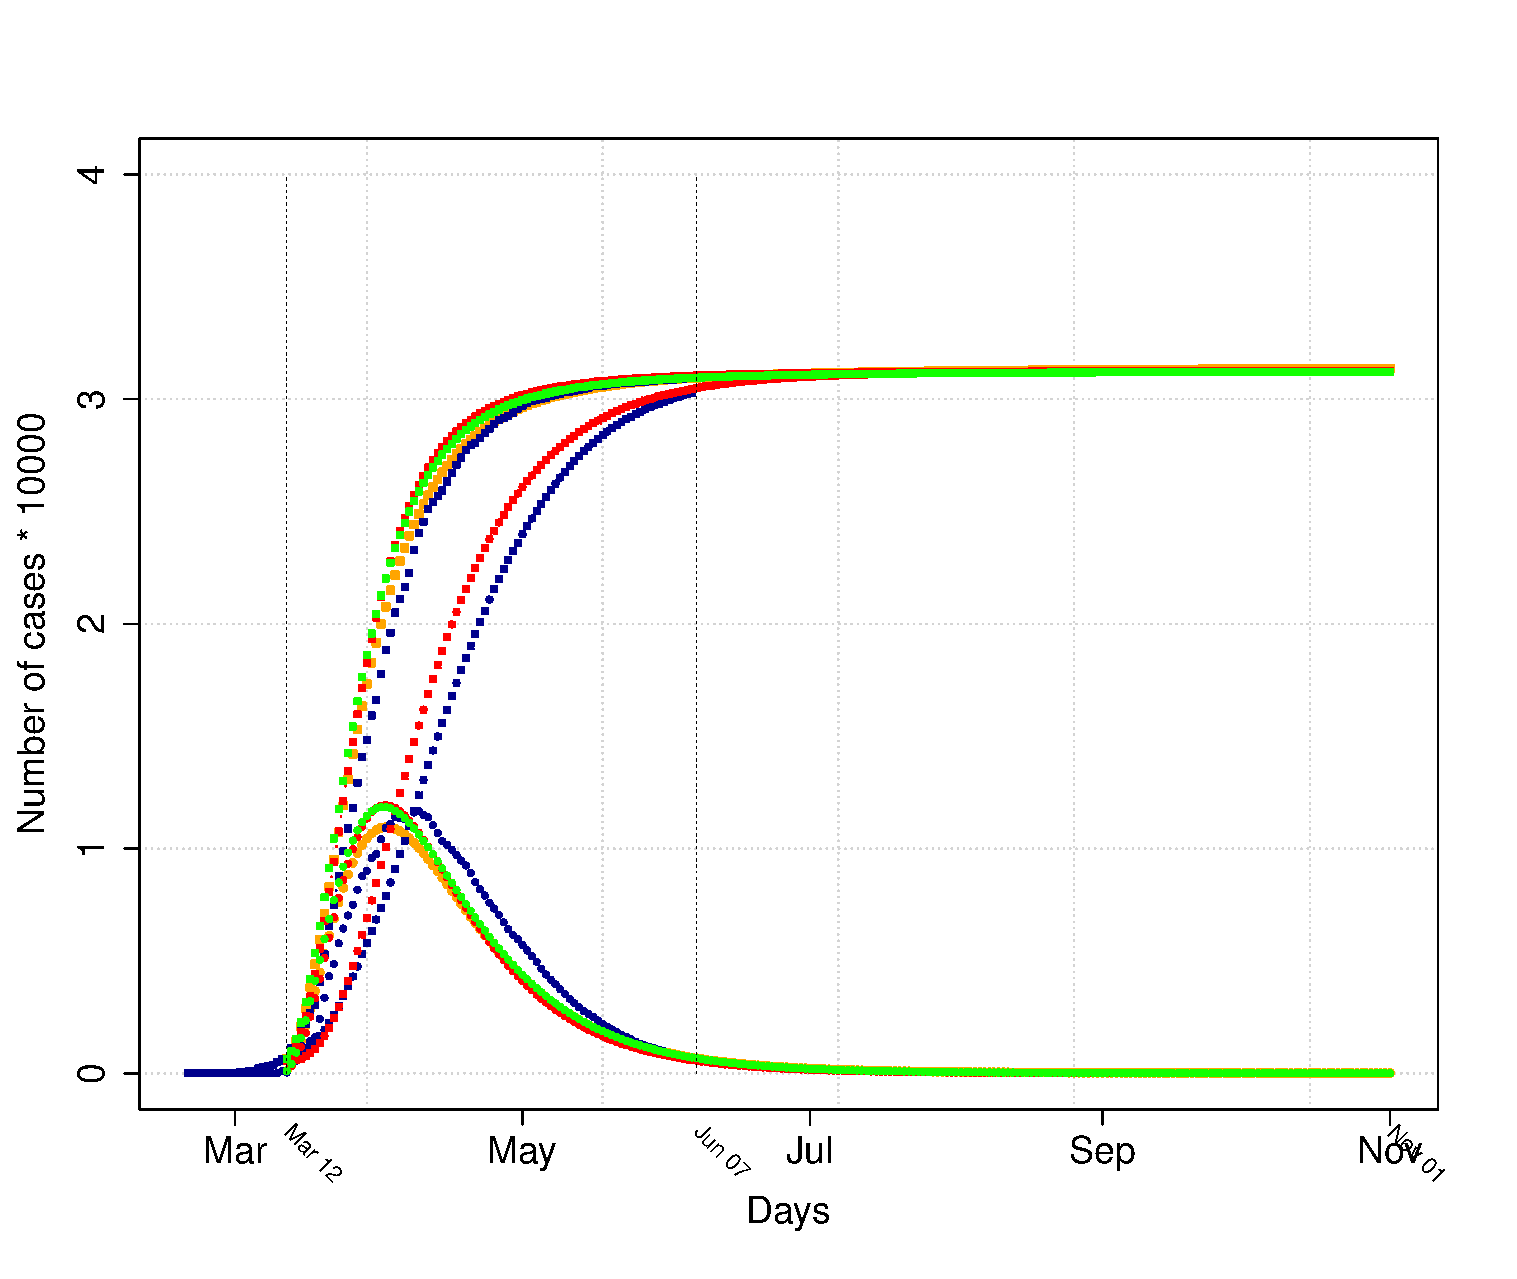
\includegraphics[width=2.5in,height=2in]{swiss_figure_a_07_06_2020.eps}}
\qquad
{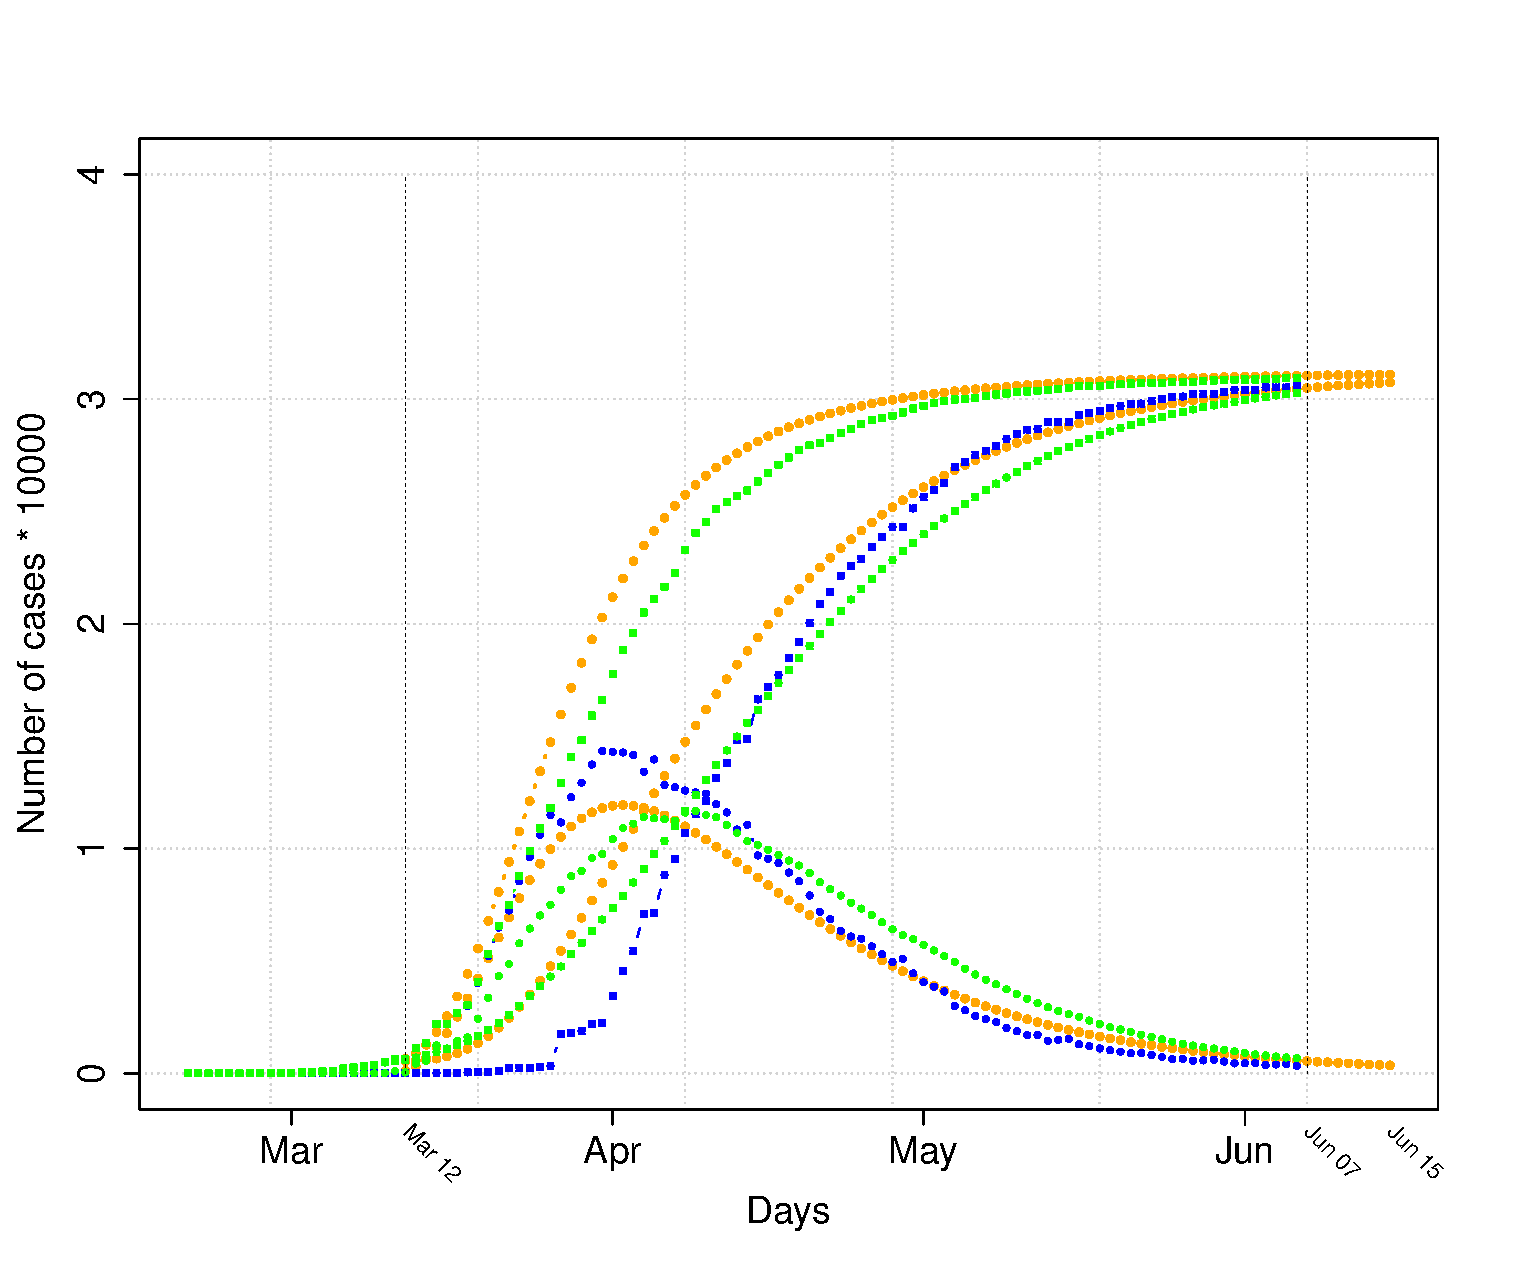
\includegraphics[width=2.5in,height=2in]{swiss_figure_b_07_06_2020.eps}}
\end{center}
\begin{center}
\caption{SIR model, data pre-processing and RTT solution, Switzerland, March to June 2020
}
\label{fig:swiss_sir_model_07_06_2020}
\end{center}
\end{figure}

\begin{figure}
\begin{center}
%\subfloat [Second-chance model and absolute standard normal]
{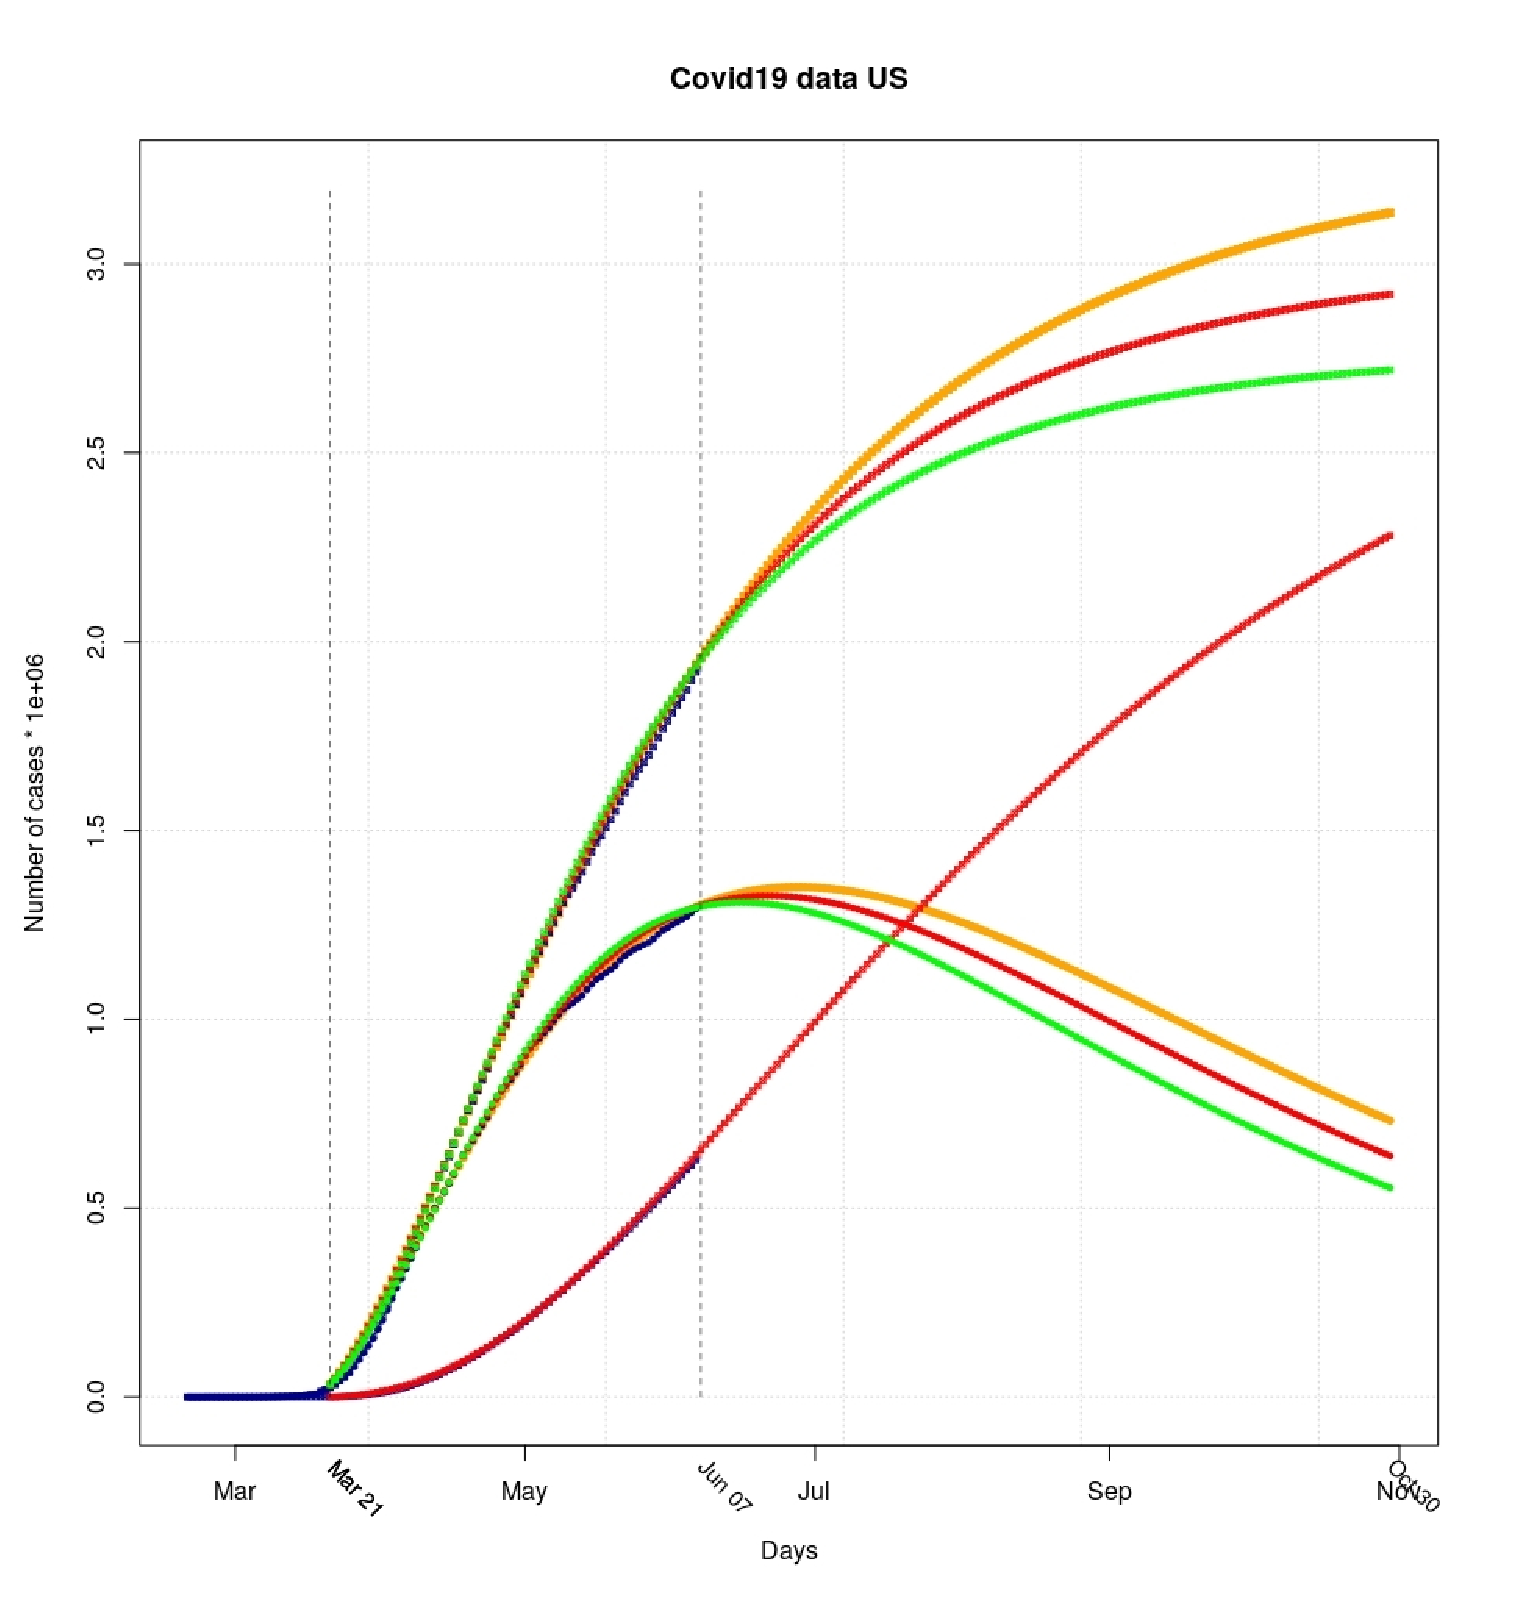
\includegraphics[width=2.5in,height=2in]{usa_figure_a_07_06_2020.eps}}
\qquad
{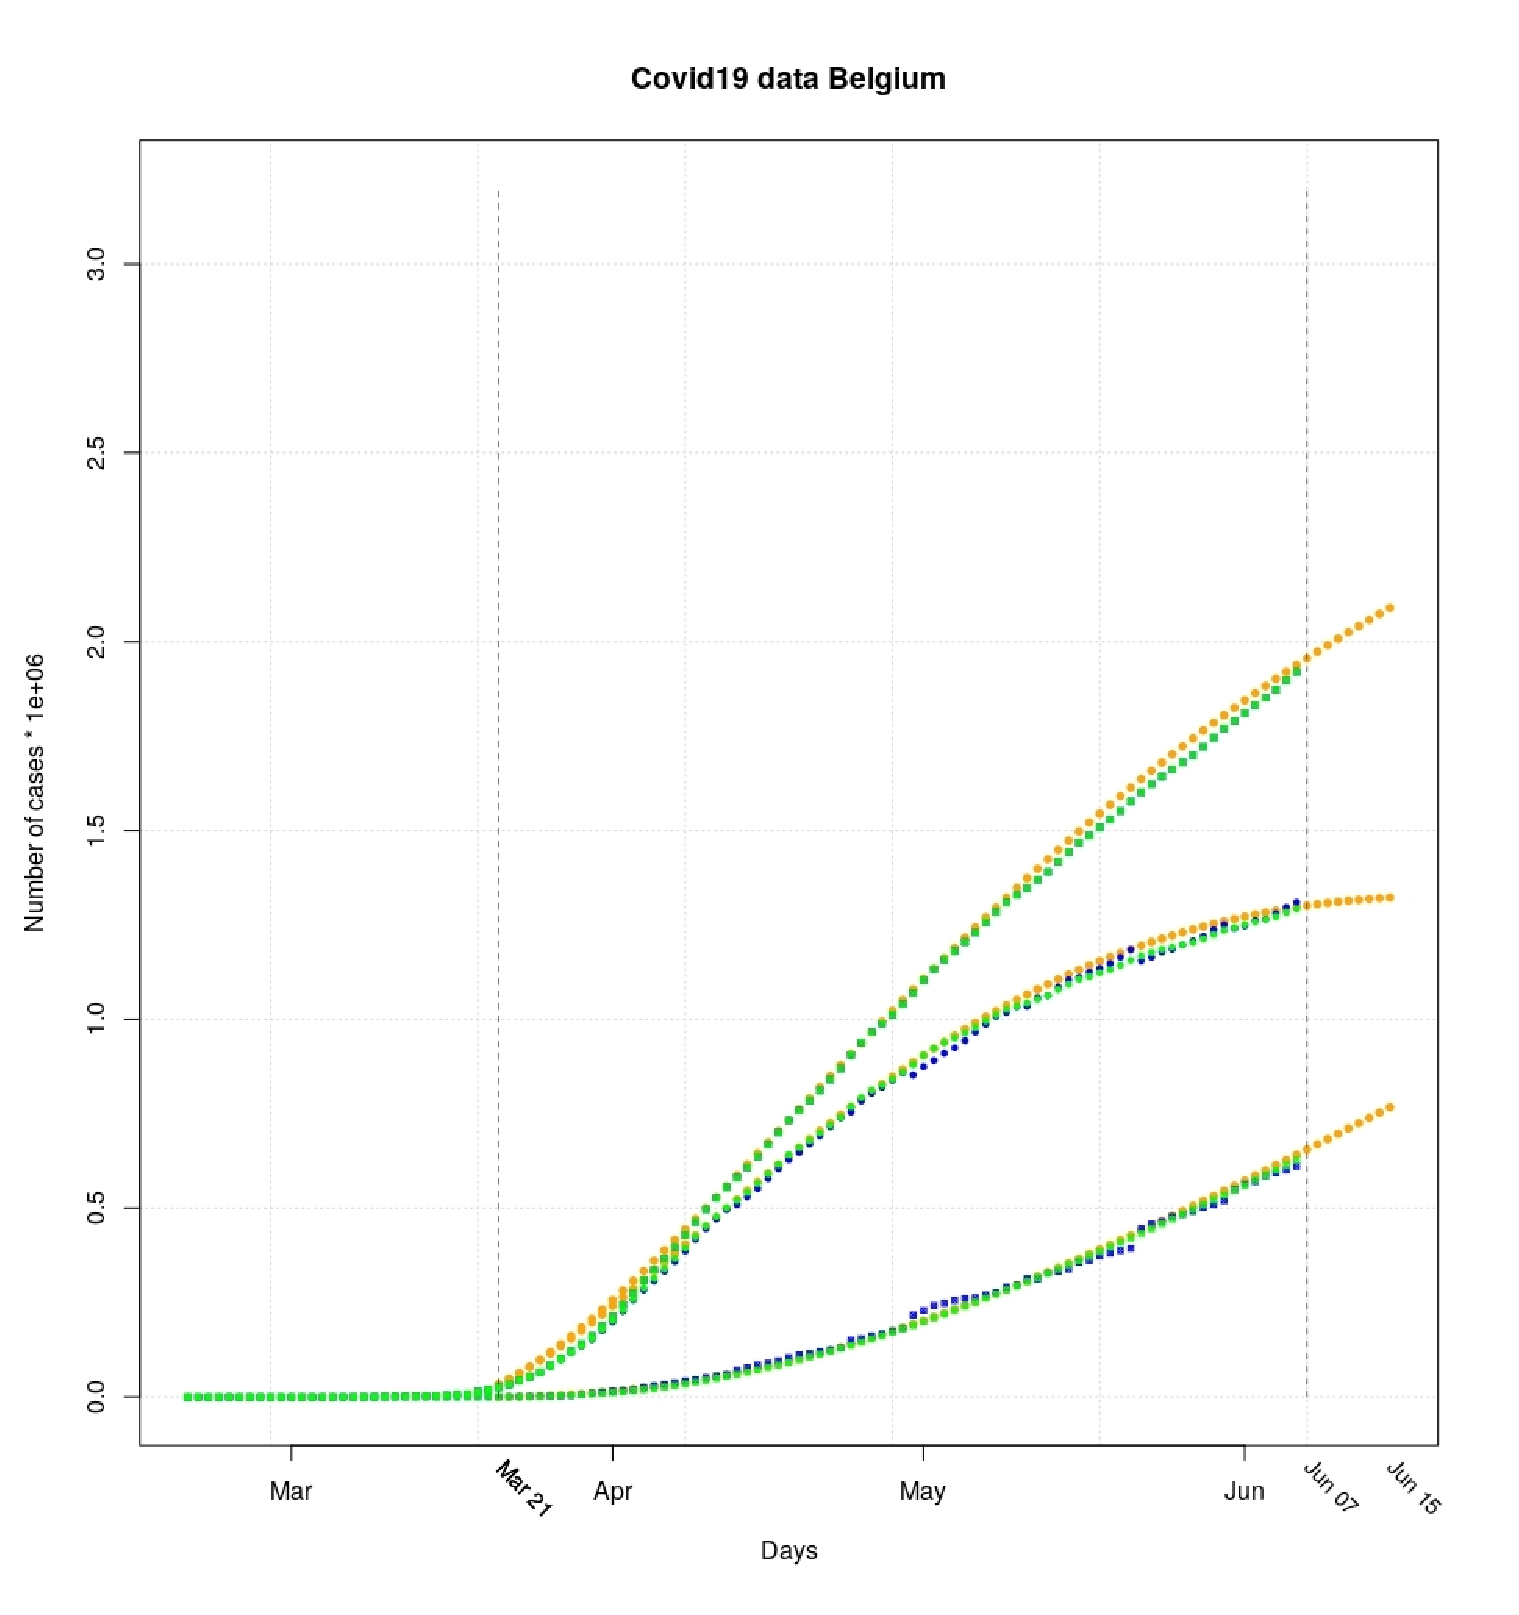
\includegraphics[width=2.5in,height=2in]{usa_figure_b_07_06_2020.eps}}
\end{center}
\begin{center}
\caption{SIR model, data pre-processing and RTT solution, USA, March to June 2020
}
\label{fig:usa_sir_model_07_06_2020}
\end{center}
\end{figure}



\begin{figure}[H]
\begin{center}
%\subfloat [Second-chance model and absolute standard normal]
{\includegraphics[width=2.5in,height=2in]{chile.eps}}
\qquad
{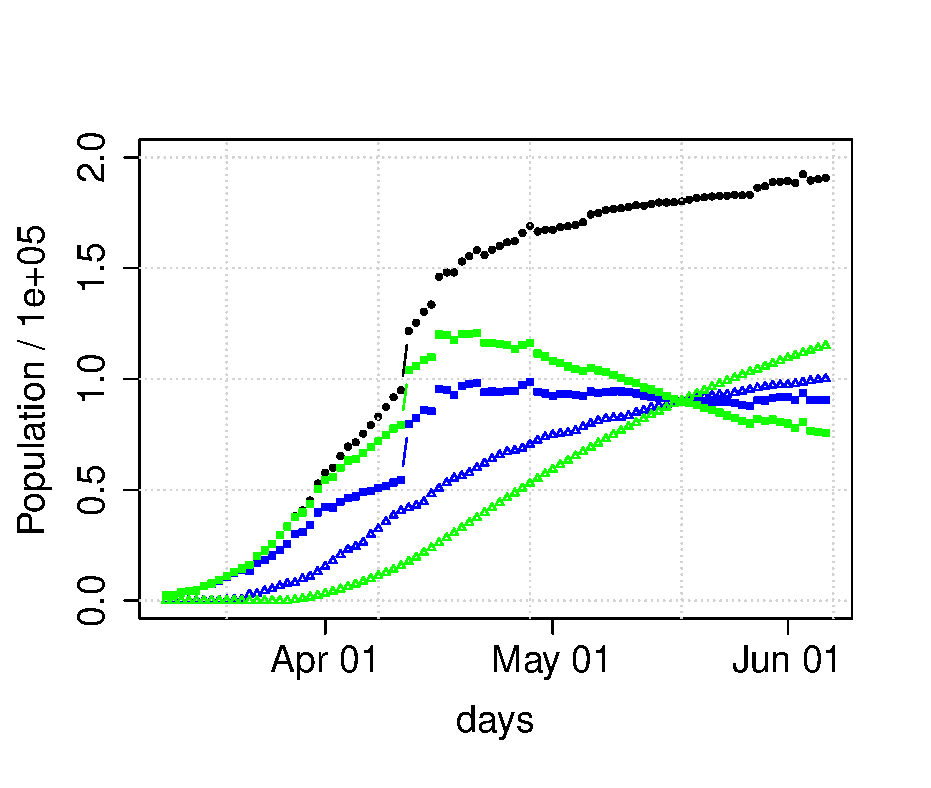
\includegraphics[width=2.5in,height=2in]{france.eps}}
\qquad
{\includegraphics[width=2.5in,height=2in]{india.eps}}
\qquad
{\includegraphics[width=2.5in,height=2in]{iran.eps}}
\end{center}
\begin{center}
\caption{Data pre-processing: Raw in blue, modified in green. Chile (top left), France (top right), India (bottom left) and Iran (bottom right), March to June 2020
}
\label{fig:chile_france_india_iran_07_06_2020}
\end{center}
\end{figure}

\begin{figure}[H]
    \begin{center}
%\subfloat [Second-chance model and absolute standard normal]
        {\includegraphics[width=2.5in,height=2in]{israel.eps}}
        \qquad
        {\includegraphics[width=2.5in,height=2in]{peru.eps}}
        \qquad
    {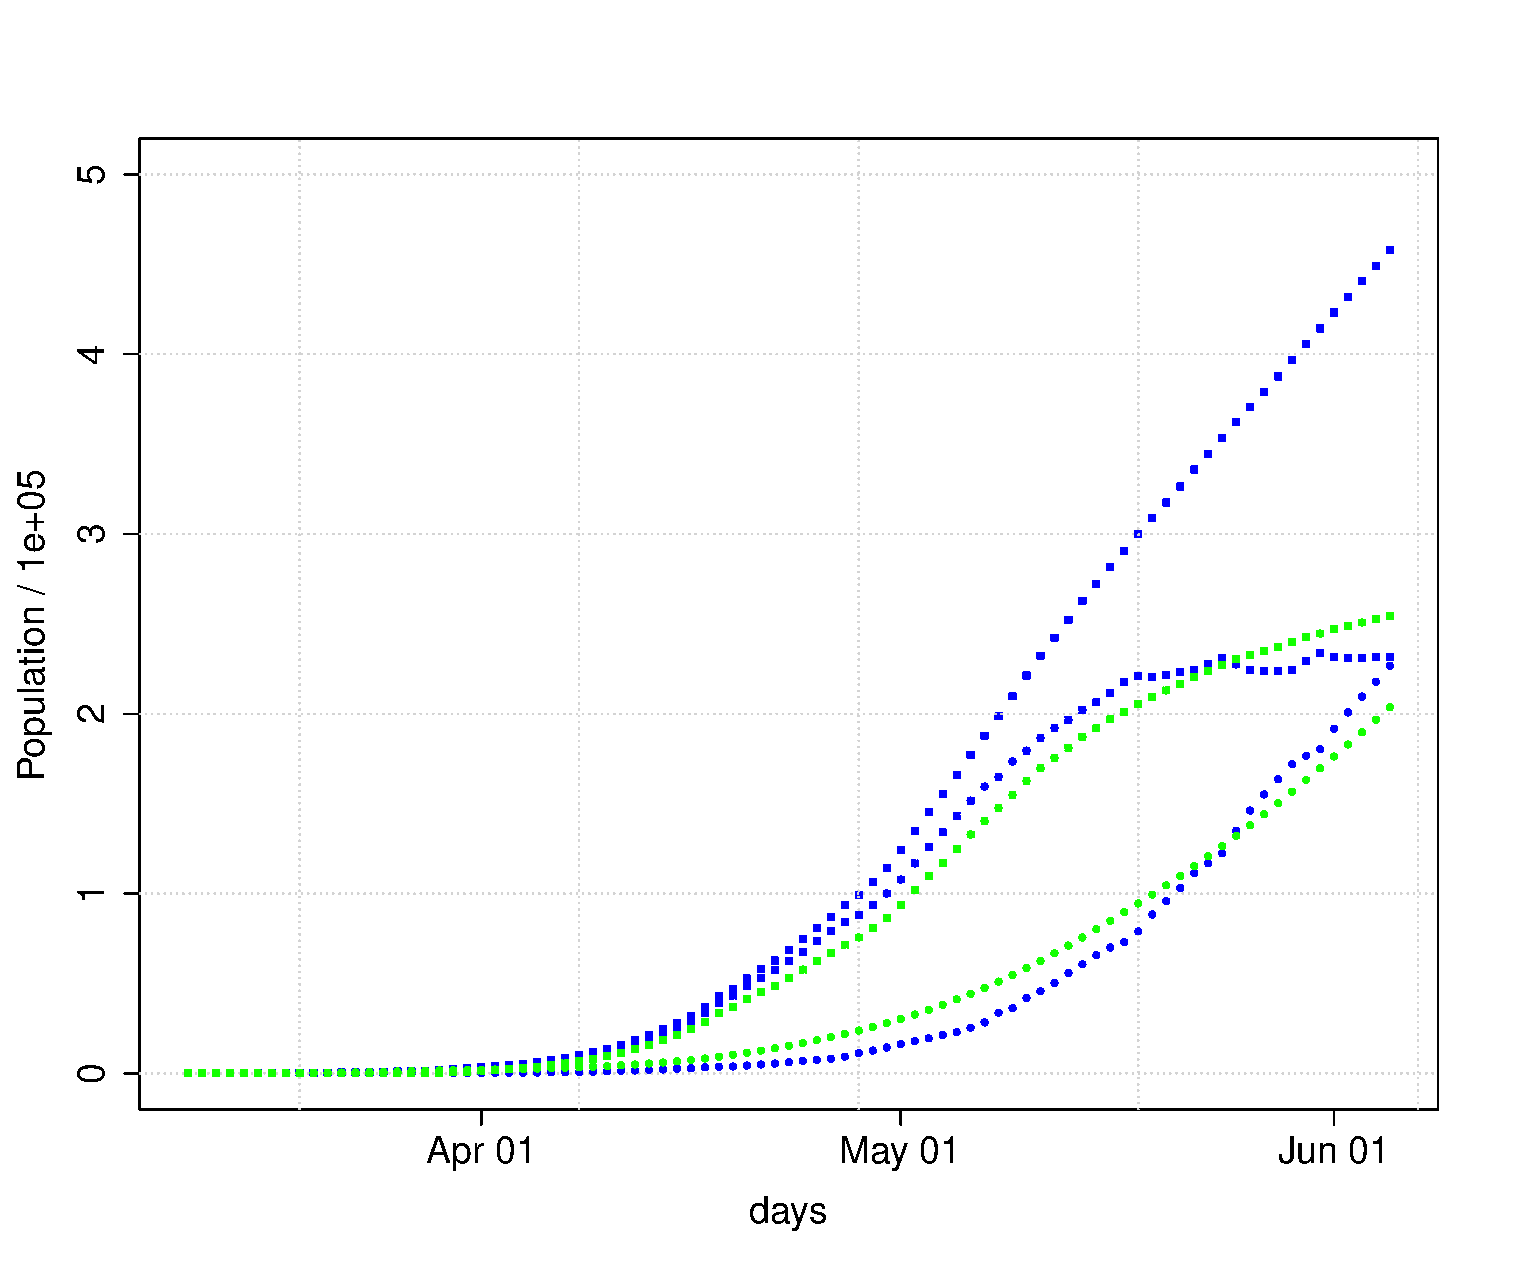
\includegraphics[width=2.5in,height=2in]{russia.eps}}
    \qquad
    {\includegraphics[width=2.5in,height=2in]{turkey.eps}}
    \end{center}
    \begin{center}
    \caption{Data pre-processing: Raw in blue, modified in green. Israel (top left), Peru (top right), Russia (bottom left) and Turkey (bottom right), March to June 2020
    }
\label{fig:israel_peru_russia_turkey_07_06_2020}
    \end{center}
\end{figure}


\begin{figure}[H]
    \begin{center}
%\subfloat [Second-chance model and absolute standard normal]
        {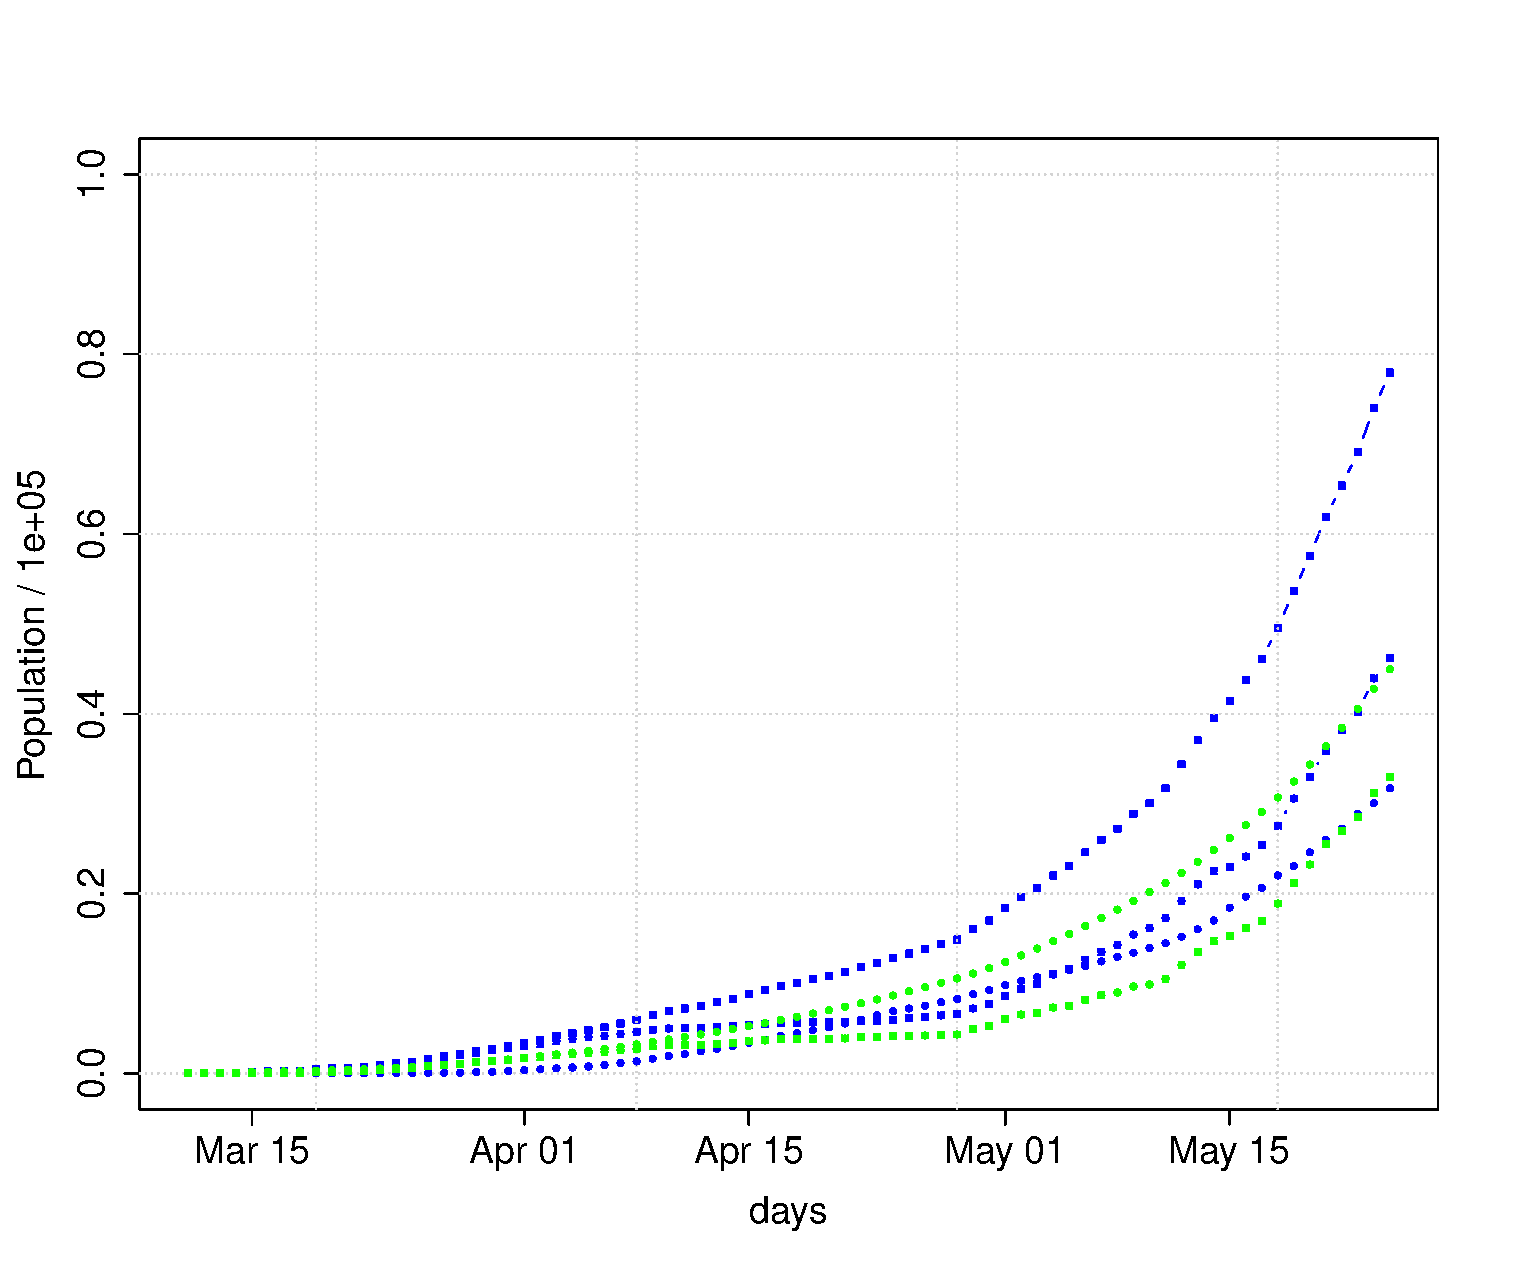
\includegraphics[width=2.5in,height=2in]{chile_25_05_2020.eps}}
        \qquad
        {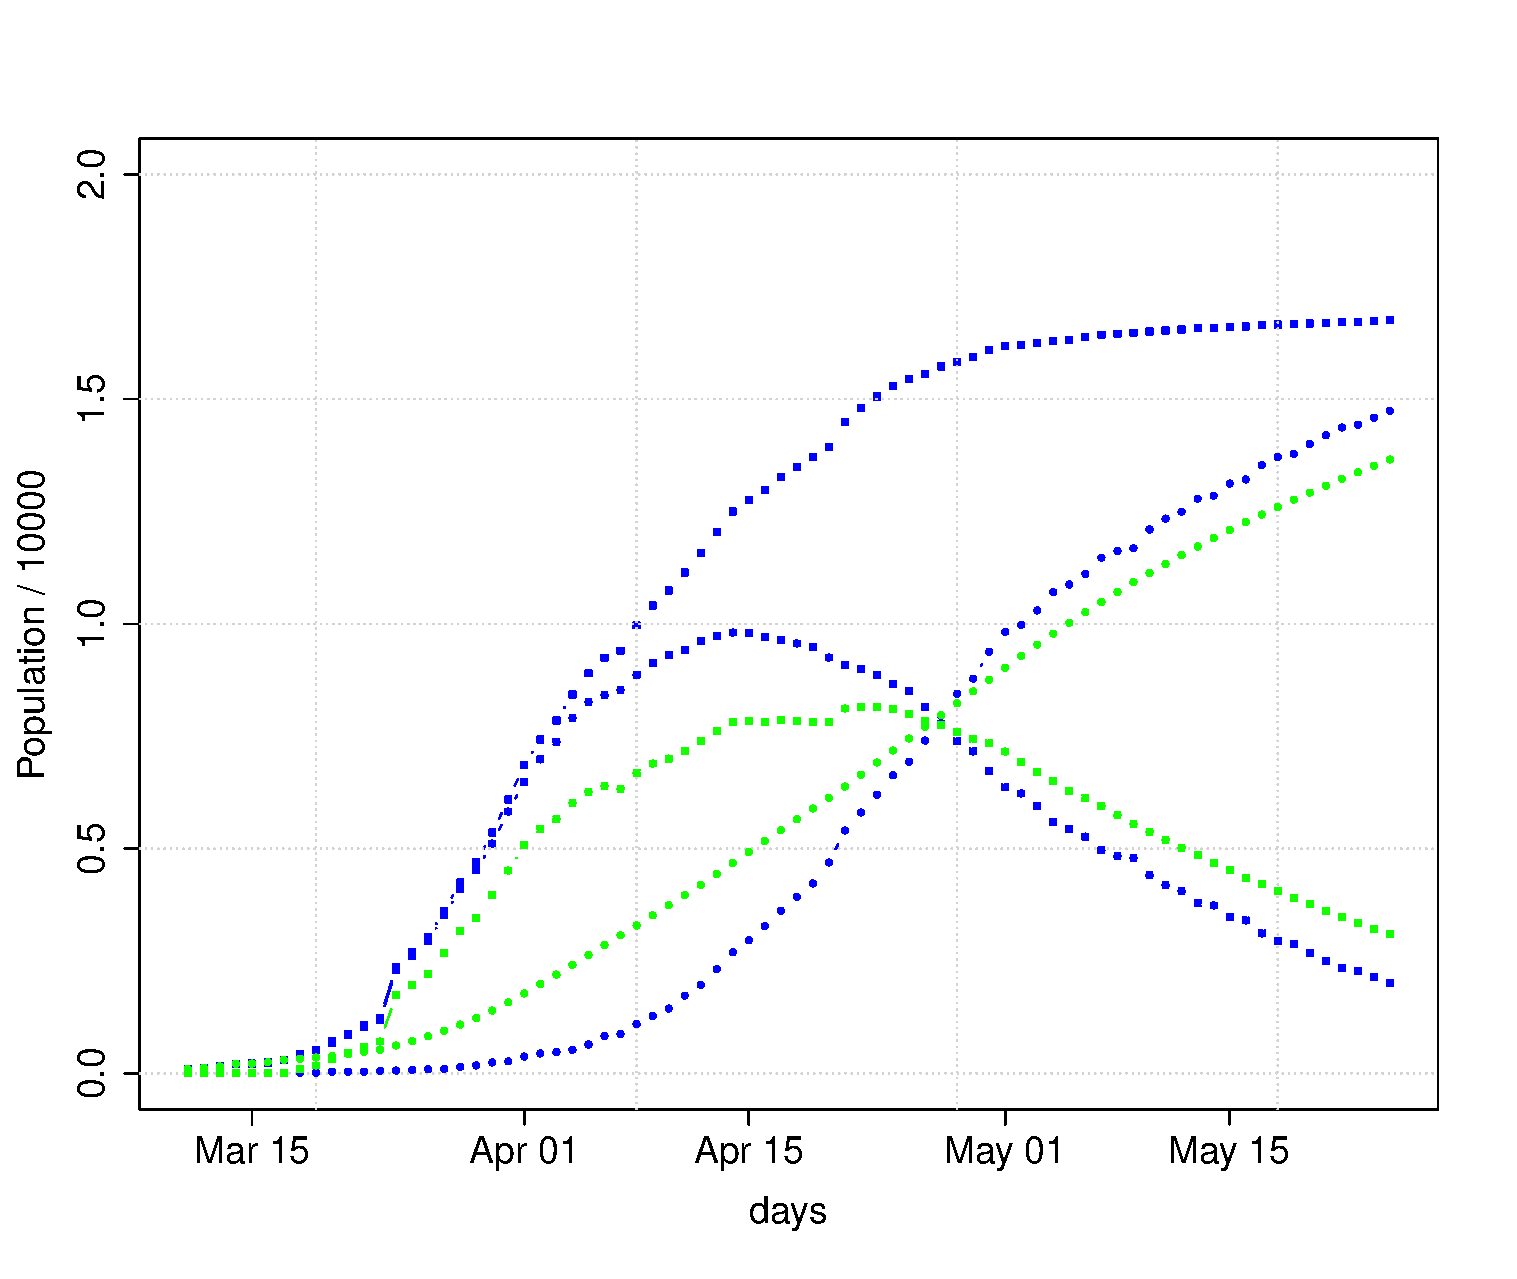
\includegraphics[width=2.5in,height=2in]{israel_25_05_2020.eps}}
    \end{center}
    \begin{center}
    \caption{Data pre-processing: Raw in blue, modified in green. Chile (left) and Israel (right), March to May 25th 2020
    }
\label{fig:chile_and_israel_25_05_2020}
    \end{center}
\end{figure}

\newpage

\noindent {Appendix: A connection between RTT and SDE}

\bigskip

\noindent If $X$ and $R$ are diffusions and time increments are small enough, local behavior is BN with drift given by the integrands in the SIR ODE and some diffusion coefficients. As such, the incremental random times $\tau$ are first passage times of BM, first hitting times of constant heights $D$, with well known density functions, that should have been used to build the likelihood model. In the benefit of simplicity and the ease with which the normal approximation handles dependent random times, we opted for the Gaussian inaccuracy.

\bigskip

\noindent Let any of the two BM $B_t$ dealt with have local drift $\mu>0$ and standard deviation $\sigma$. Since $B_t - \mu t$ and $(B_t - \mu t)^2 - \sigma^2 t$ are mean-zero Martingales, their expected values at $\tau$ are zero too. Hence, $\tau$ has mean ${D \over \mu}$ and variance ${{\sigma^2 D} \over {\mu^3}}$. Since for RTT $\tau$ has mean $1$ and constant variance, $\sigma$ must be proportional to $\mu$. So the SDE corresponding to the SIR ODE has diffusion term proportional to the drift term. Under the assumption that sampling is frequent enough, the Fokker-Planck equations lead to a likelihood function close to the Gaussian likelihood with exponential term (for $X$)
$$
\exp\{-{1 \over {2 \sigma^2}}\sum ({{X(i+1)-X(i)} \over {{x({{i+1} \over \delta})-x({{i} \over \delta})}b}}-1)^2\}
$$
and the corresponding denominator. ${{x({{i+1} \over \delta})-x({{i} \over \delta})}}$ can be replaced by the mid-interval differentials.

\section*{Acknowledgements}

Thanks are due to Ilan Eshel from prompting this study and to Vahid
Bokharaie, Amit Huppert, Eytan Ruppin, Laura Sacerdote and David Steinberg for helpful suggestions.

The data analyzed in this work is taken from the COVID-19 Data Repository by
the Center for Systems Science and Engineering (CSSE) at Johns Hopkins
University.

%\end{\huge}

\baselineskip= 28pt

\begin{thebibliography}{99}

\bibitem{Alon} Alon N. (2019), The effect of drift change on Skorohod embedded
distribution with applications in Finance. Master’s Thesis, Tel Aviv
University

\bibitem{Bassanetal} Bassan, B., Marcus, R., Meilijson, I. and Talpaz, H. (1997). Parameter erstimation in differential equations, using random time transformations. {\em Journal of the Italian Statistical Society}, {\bf 6}, 177--199.

\bibitem{Cuadras} Fortiana, J. and Cuadras, C. M. (1997). A family of matrices, the
discretized brownian bridge, and distance-based regression. {\em Linear
Algebra and its Applications}, {\bf 264}, 173–-188.

\bibitem{AAA} Grenfell, B.T., Bj{\o}rnstad, O.N. and Filkenst\"{a}dt, B. A. (2002) Dynamics of Measles epidemics: scaling, noise, determinism and predictability with the TSIR model. {\em Ecological Monographs}, {\bf 72(2)}, 185-–202.

\bibitem{Karatzas} Karatzas, I. and Shreve, S. E. (1998). {\em Brownian Motion and Stochastic Calculus}. Graduate texts in Mathematics, Springer.

\bibitem{Kermack}  Kermack, W. O., McKendrick, A. G. (1927). A Contribution to the Mathematical Theory of Epidemics. {\em Proceedings of the Royal Society A}, {\bf 115 (772)}, 700-–721.

\bibitem{Krengel} Krengel, U. (1985). {\em Ergodic theorems}. de Gruyter.

\bibitem{Murphy} Murphy, S. A. and  Van Der Vaart, A. W. (2000). On Profile Likelihood. {\em Journal of the American Statistical Association}.
\end{thebibliography}

\end{document}


